\documentclass[UTF8]{ctexart}
\usepackage{geometry}
\usepackage{indentfirst}
\usepackage{hyperref}
\usepackage{harpoon}
\usepackage{amsmath}
\usepackage{amssymb}
\usepackage{graphicx}
\usepackage{float}
\usepackage{subfigure}
\usepackage{multirow}
\usepackage{array}
\usepackage{tikz}
\usetikzlibrary{arrows, shapes, positioning, calc}
\geometry{a4paper, left=1cm, right=1cm, top=2cm, bottom=2cm}
\setlength{\parindent}{1cm}
\renewcommand\contentsname{Content}
\title{Logistic模型}
\author{段元兴}
\date{\today}
\begin{document}
\maketitle
\thispagestyle{empty}
\setcounter{page}{1}
\newpage
\tableofcontents
\newpage
    \section{Question1}
        \begin{center}
            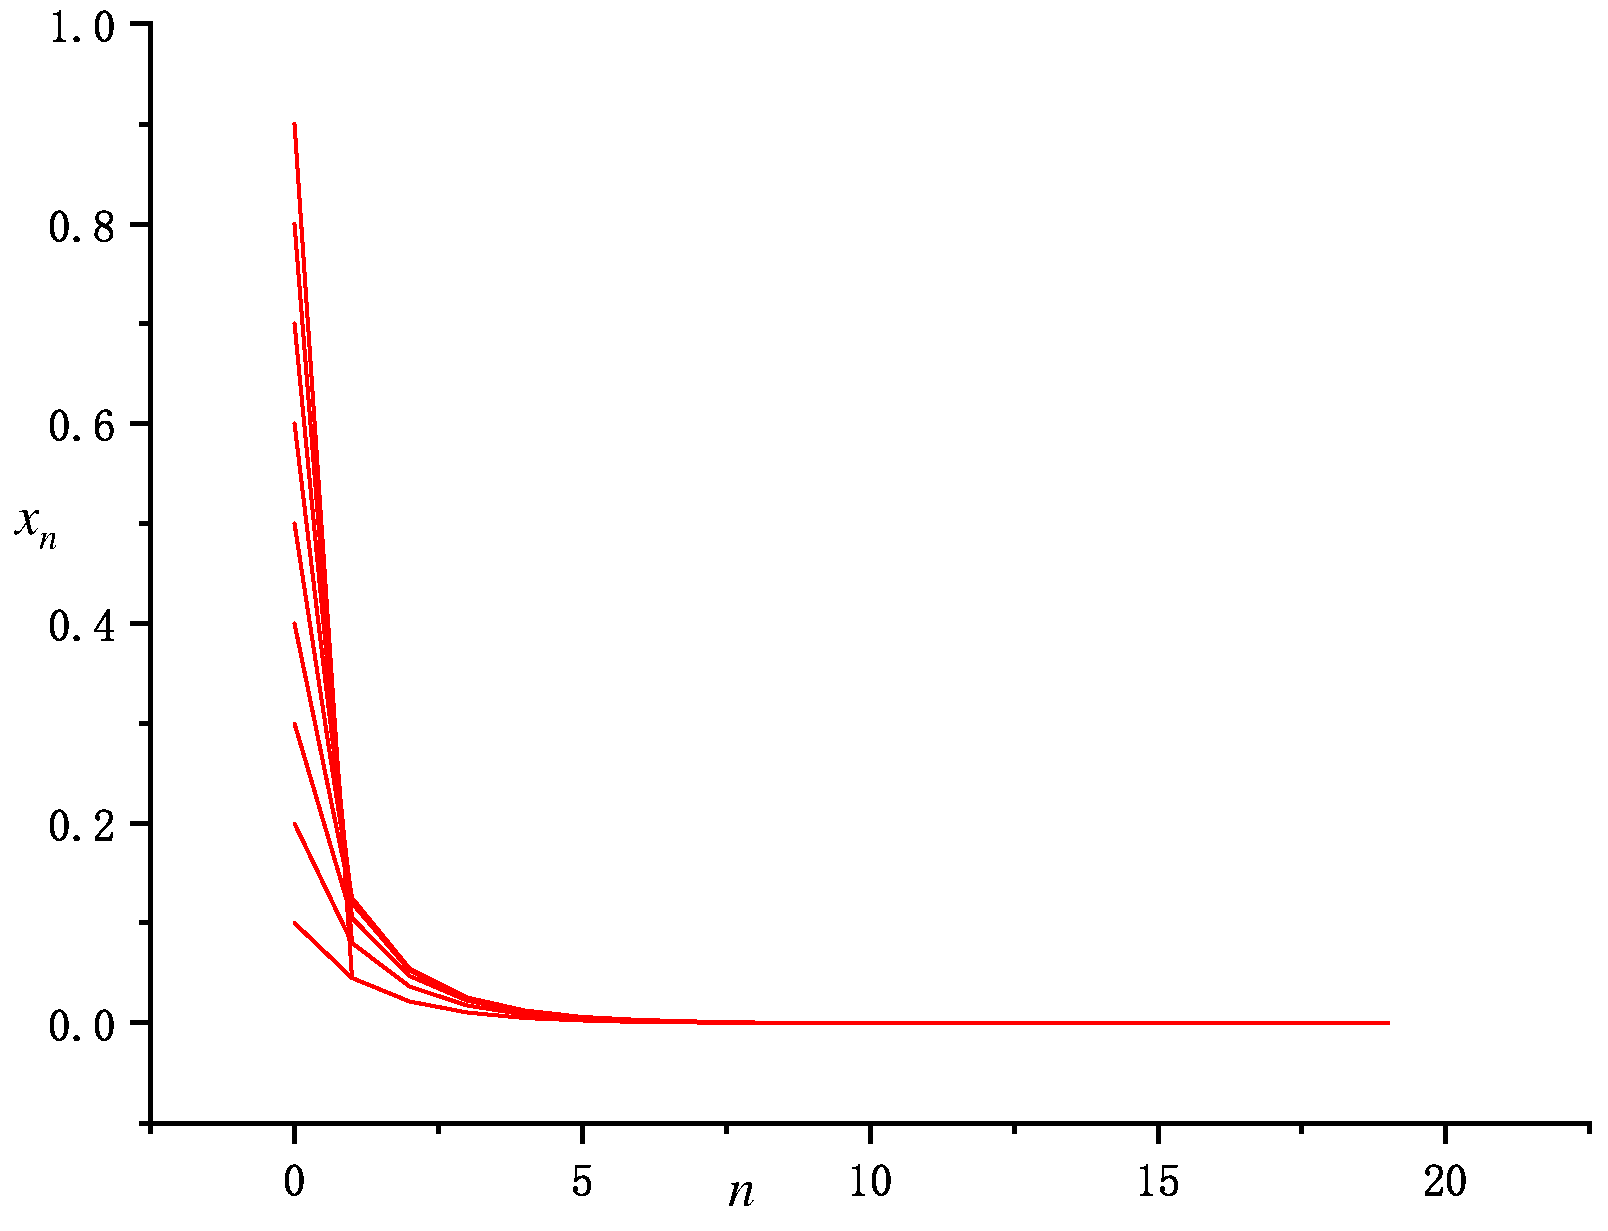
\includegraphics[width=9cm]{r0_5.pdf}
            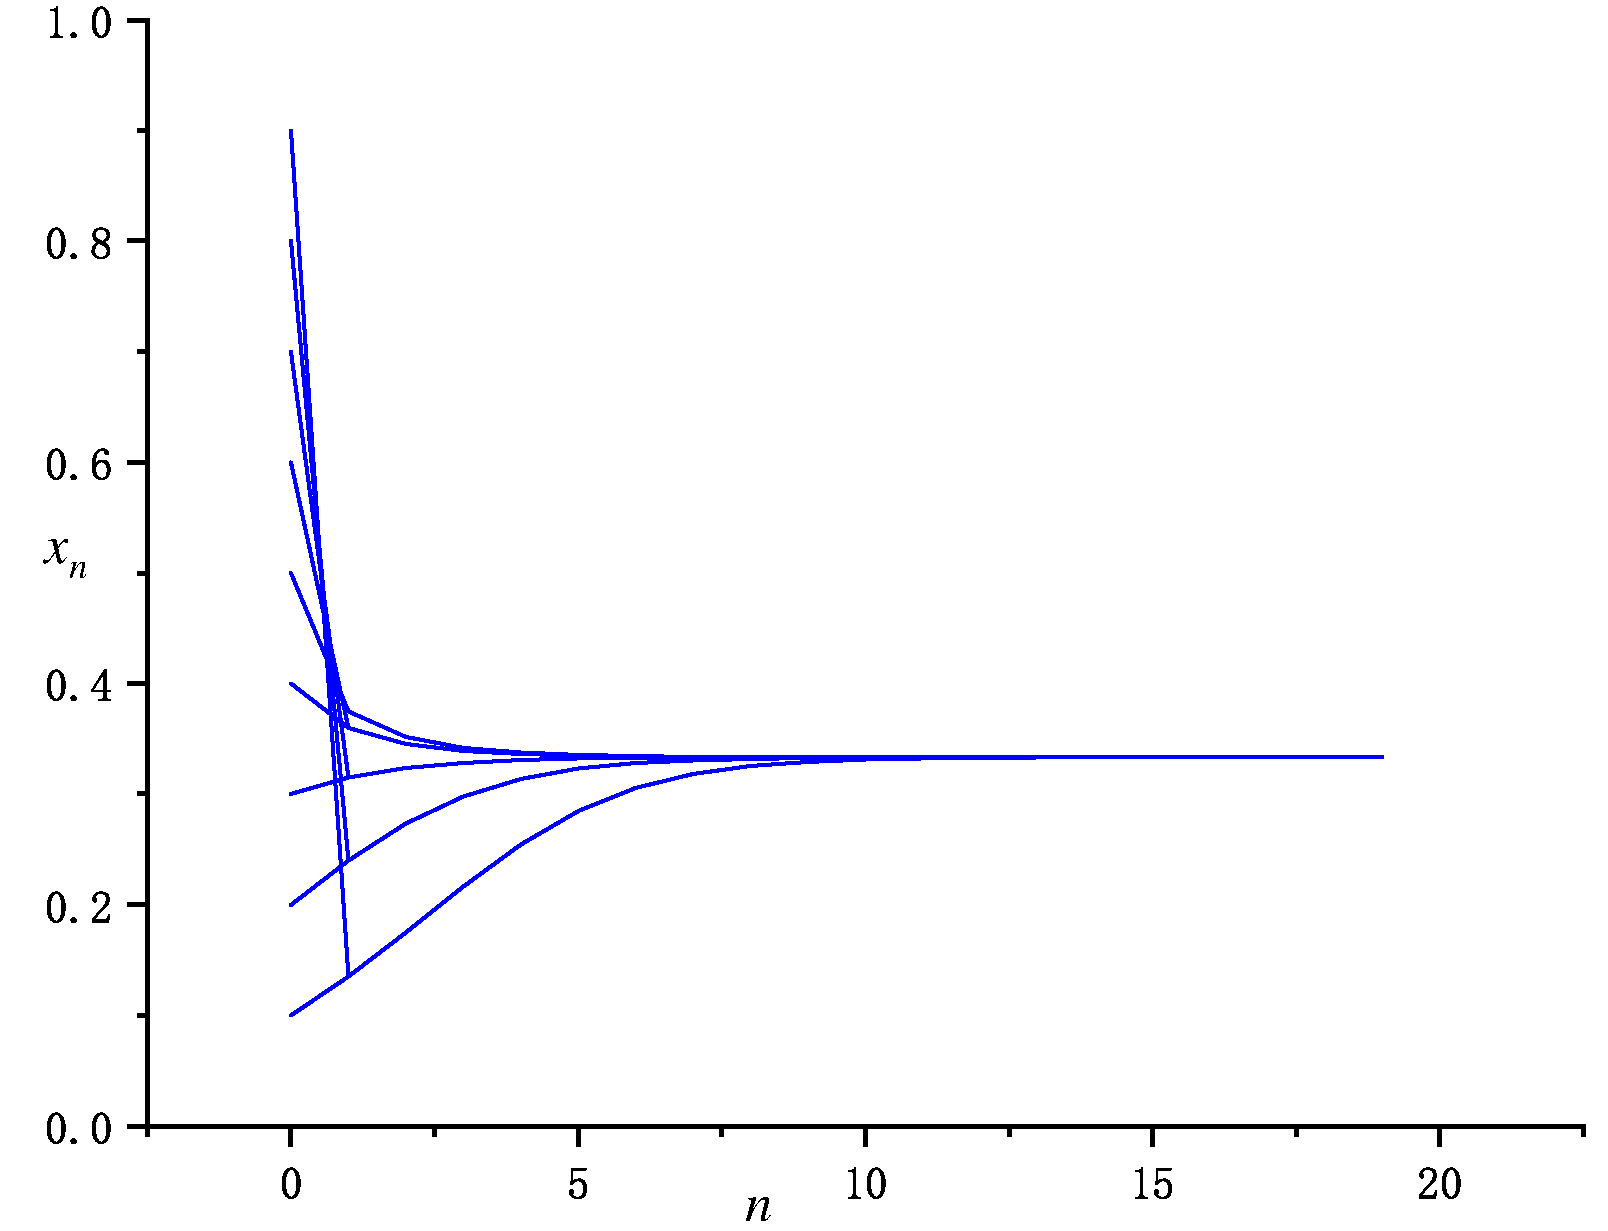
\includegraphics[width=9cm]{r1_5.pdf}
        \end{center}
    \section{Question2}
        \indent 在$x^*$附近, $\Delta x_n=x_n-x^*$带来的$\Delta x_{n+1}=x_{n+1}-x^*$的变化为:
        \begin{equation}
            \Delta x_{n+1}=x_{n+1}-x^*=f'(x^*)\left(x_n-x^*\right)=f'(x^*)\Delta x_n
        \end{equation}
        即
        \begin{equation}
            \left|\dfrac{\Delta x_{n+1}}{\Delta x_n}\right|=\left|f'(x^*)\right|.
        \end{equation}
        所以收敛于一个根的必要条件为$\left|f'(x^*)\right|<=1$. 而收敛时满足:
        \begin{equation}
            f(x^*)=x^*
        \end{equation}
        解得
        \begin{equation}
            x^*=\left\{
            \begin{array}{cc}
                0,&0<r\leqslant1\\
                1-\dfrac{1}{r},&r>1\\
            \end{array}
            \right.
        \end{equation}
        \begin{center}
            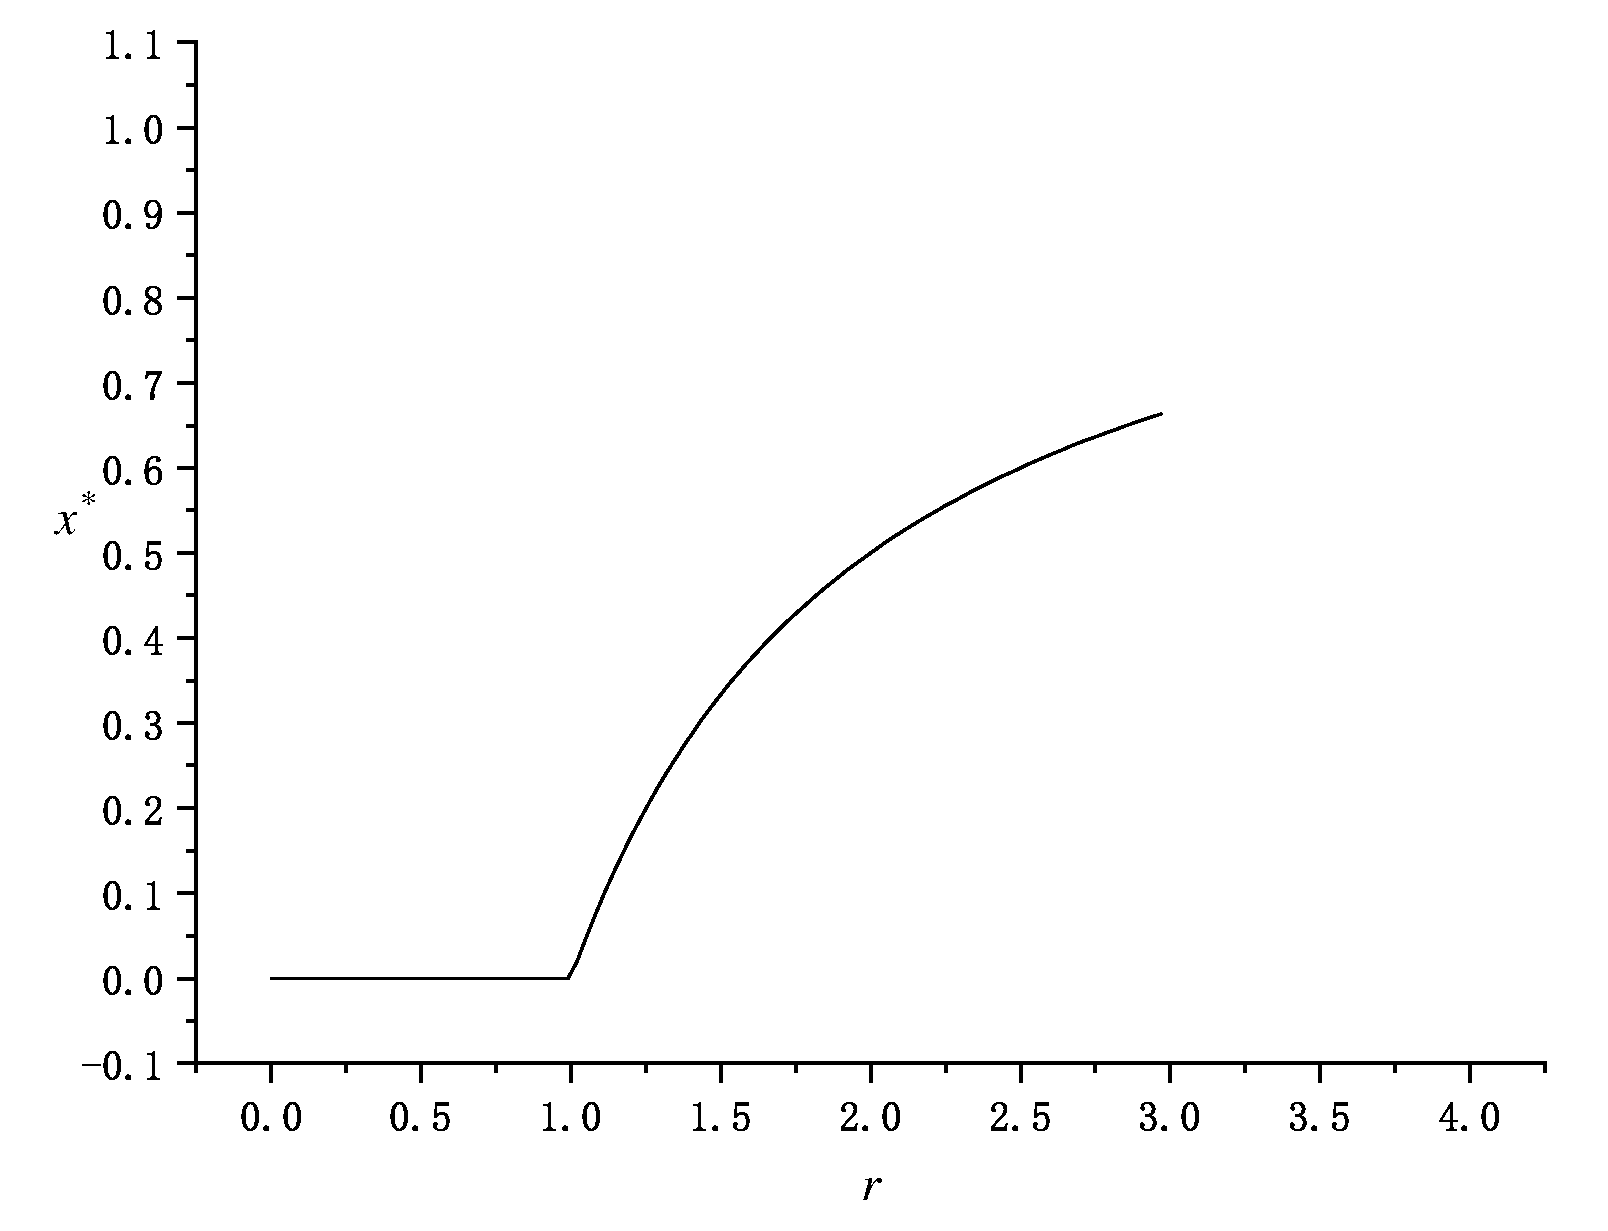
\includegraphics[width=12cm]{t1-1.pdf}
        \end{center}
        而收敛阶为1, 收敛速度为
        \begin{equation}
            f'(x^*)=\left\{
            \begin{array}{cc}
                r,&0<r\leqslant1\\
                2-r,&1<r<=3\\
            \end{array}
            \right.
        \end{equation}
    \section{Question3}
        \indent 上一问中$r_1=3$, 取$r=3.1$计算得到:
        \begin{center}
            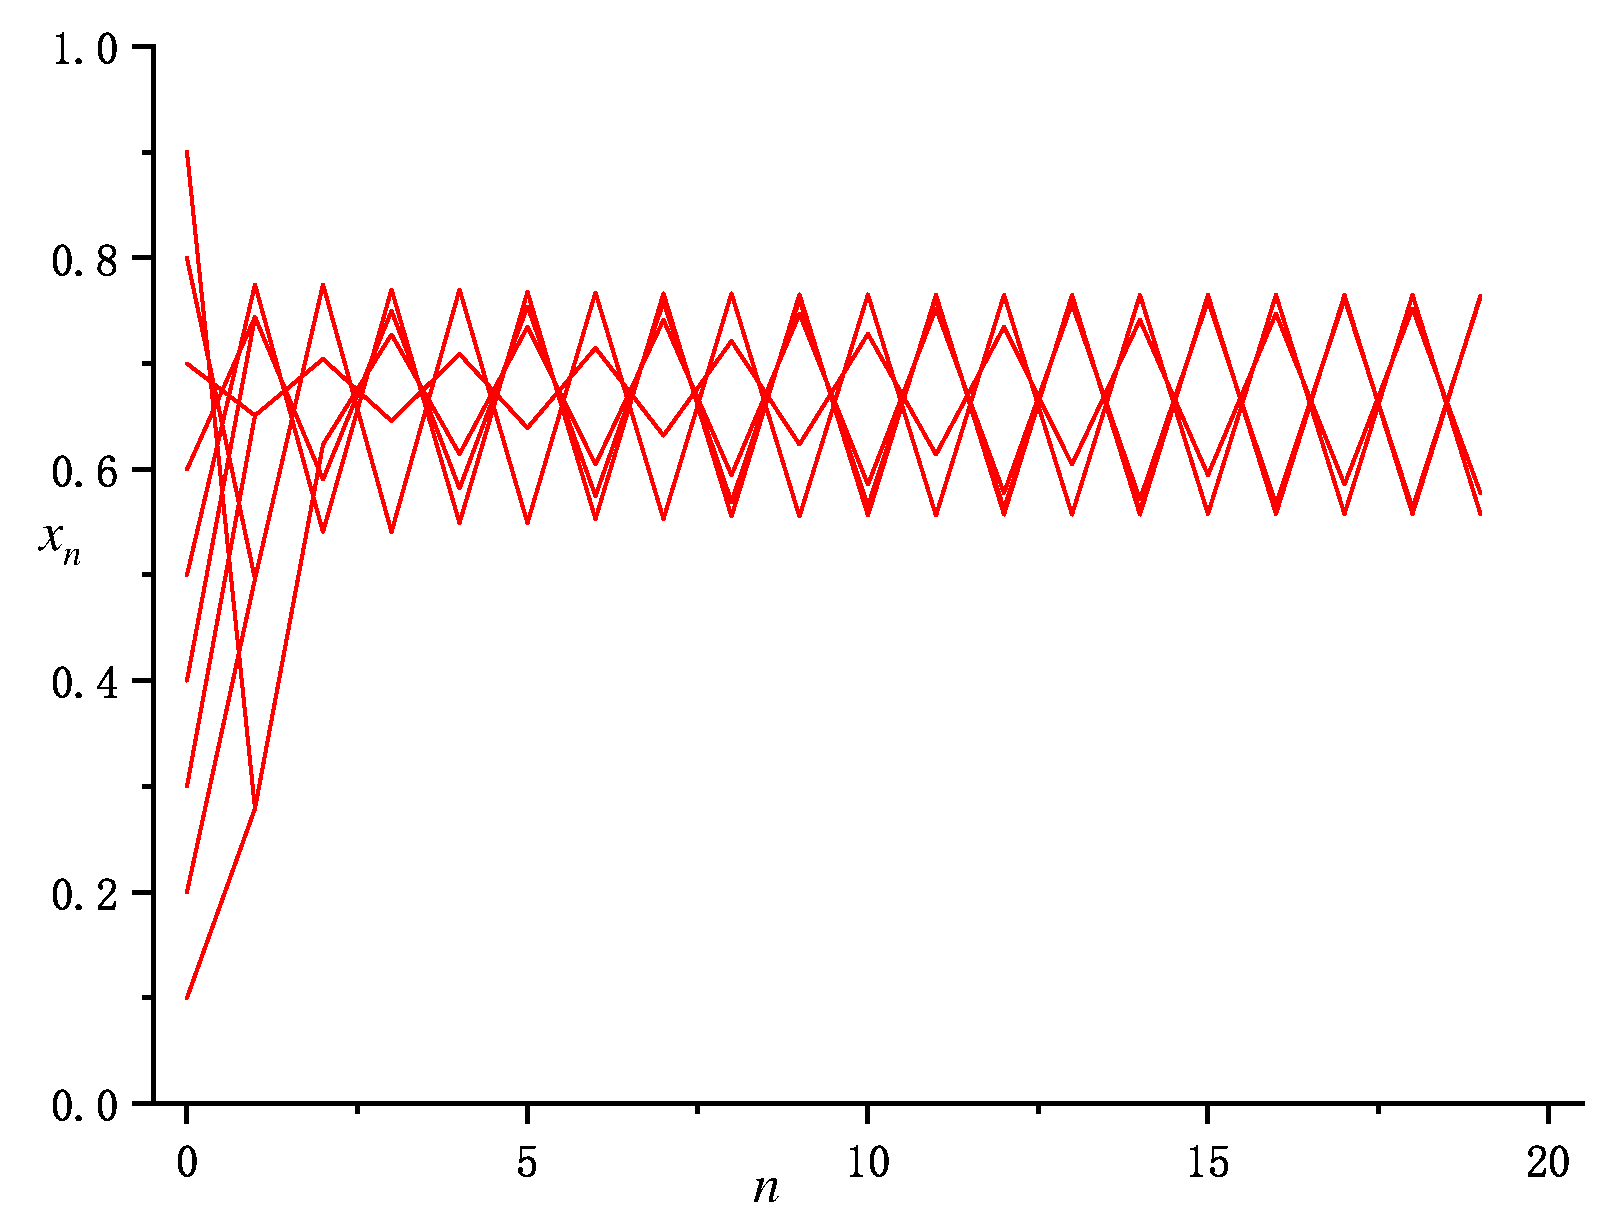
\includegraphics[width=10cm]{r3_1.pdf}
        \end{center}
        可以发现最终所有的点都振荡于0.5580141与0.7645665之间.
    \section{Question4}
        \indent 同理
        \begin{equation}
            \Delta x_{n+2}=x_{n+2}-x^*=f'(x^*_1)\Delta x_{n+1}=f'(x^*_1)f'(x^*_2)\Delta x_n
        \end{equation}
        所以收敛的必要条件为$\left|f'(x^*_1)f'(x^*_2)\right|<=1$. 而通过计算得到以下$x^*_1$和$x^*_2$关于$r(3<r<3.447)$
        的变化图像:
        \begin{center}
            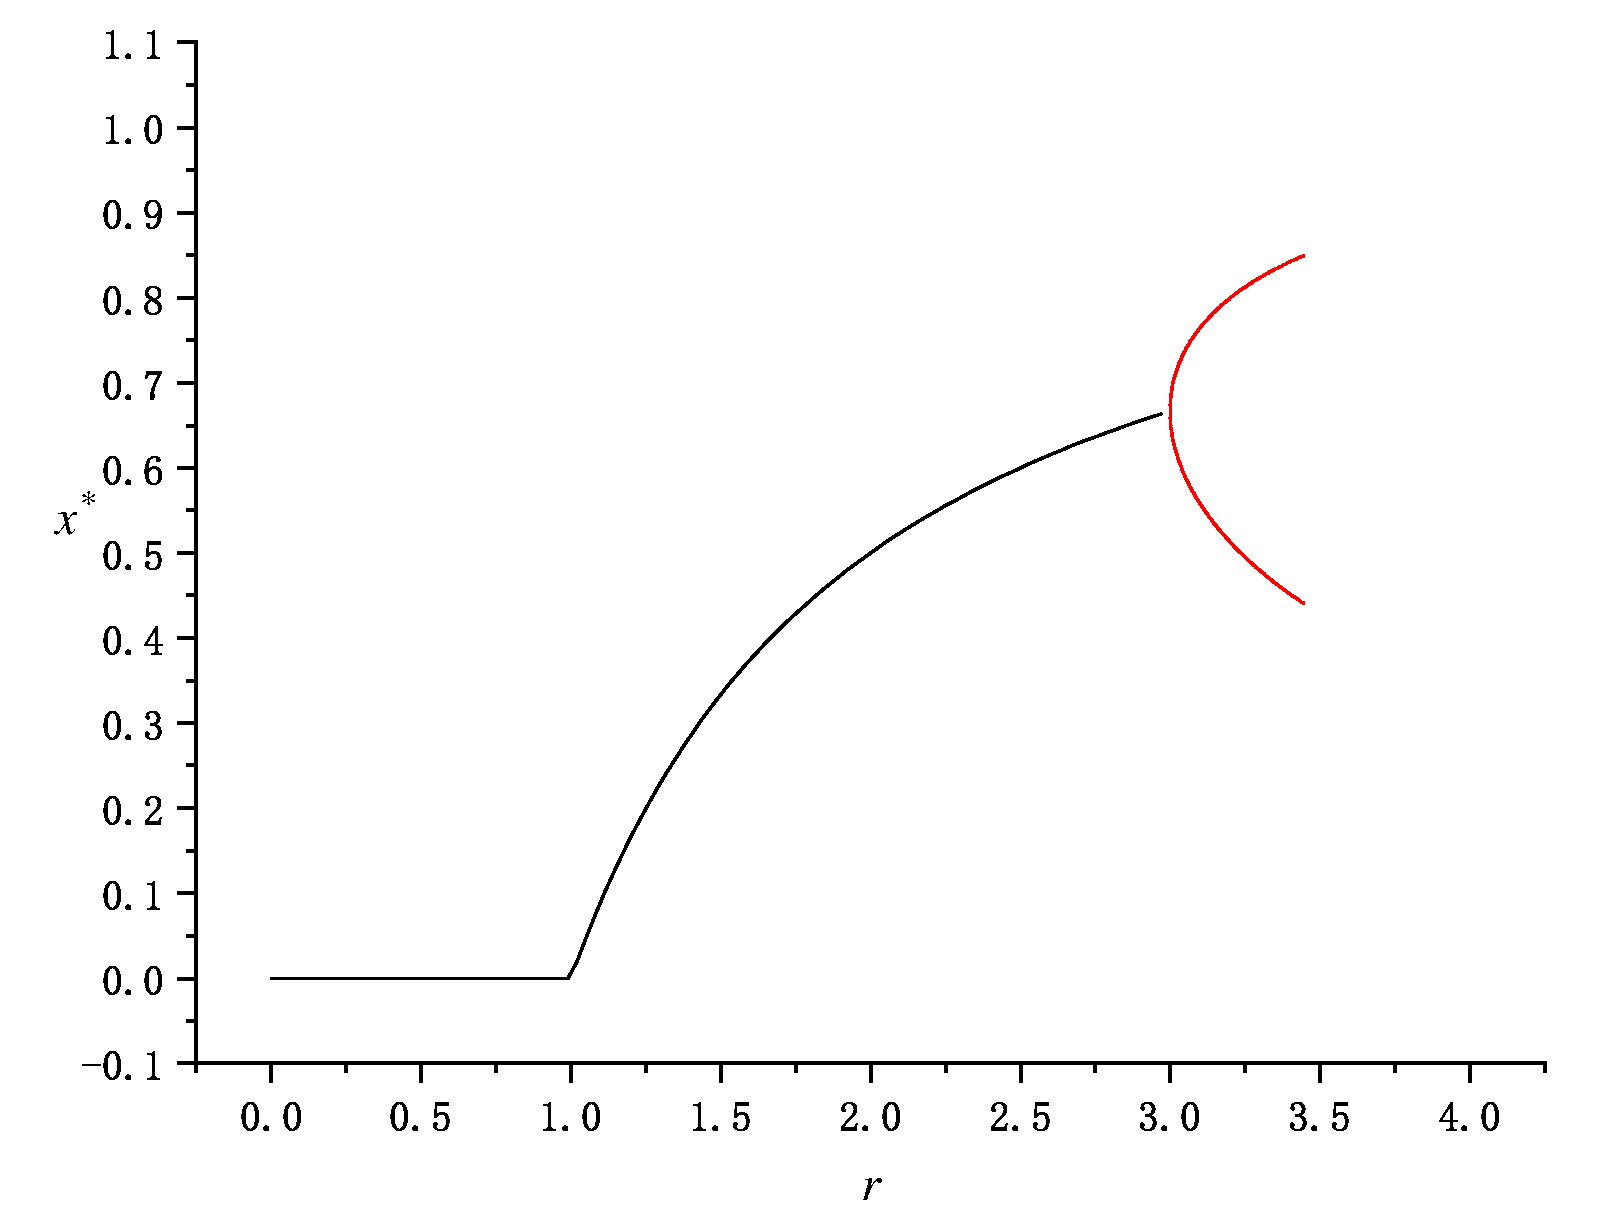
\includegraphics[width=12cm]{t1-2.pdf}
        \end{center}
    \section{Question5}
        \indent 以下是周期1-16的$x^*-r$图像:
        \begin{center}
            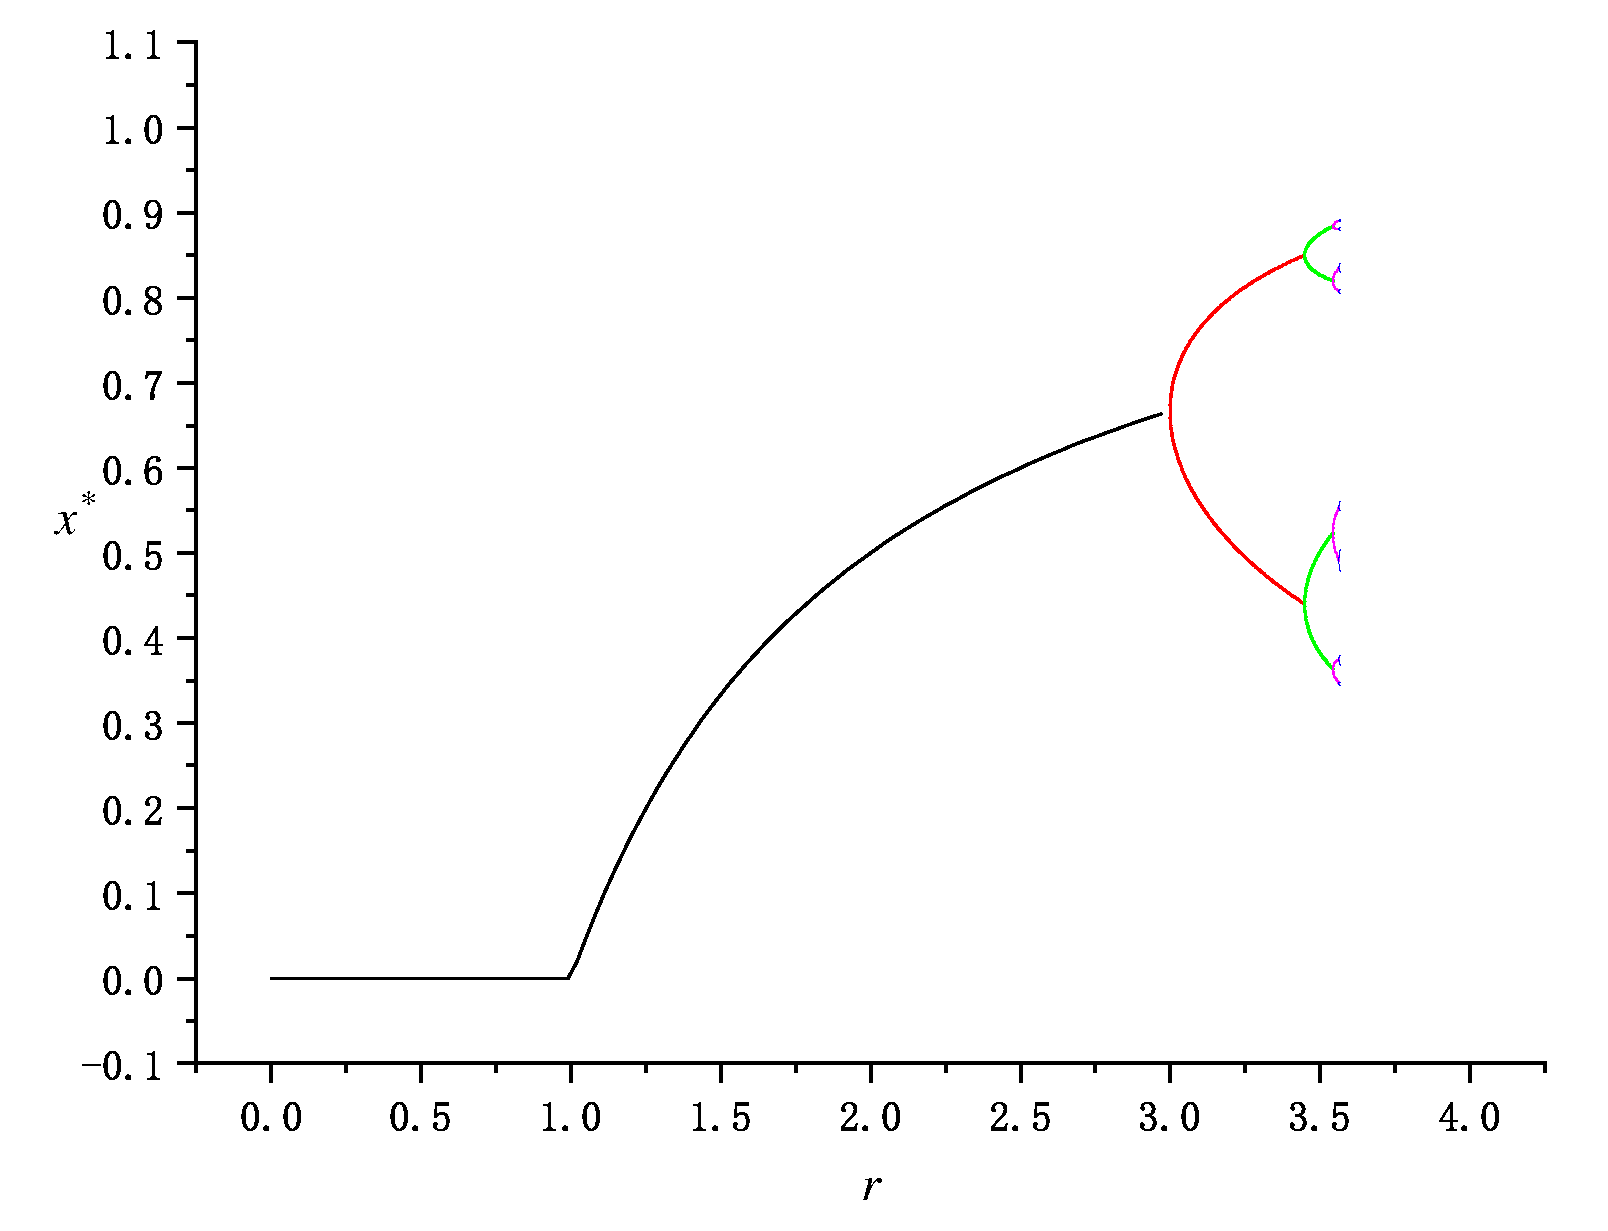
\includegraphics[width=12cm]{t1-16.pdf}
        \end{center}
        对于平均收敛速度, 我采用一个周期后$\Delta x=x-x^*$的比值$\rho=\dfrac{\Delta x_{n+1}}{\Delta x_n}$来观察,
        在每个周期区间内均匀取点得到以下图像:
        \begin{center}
            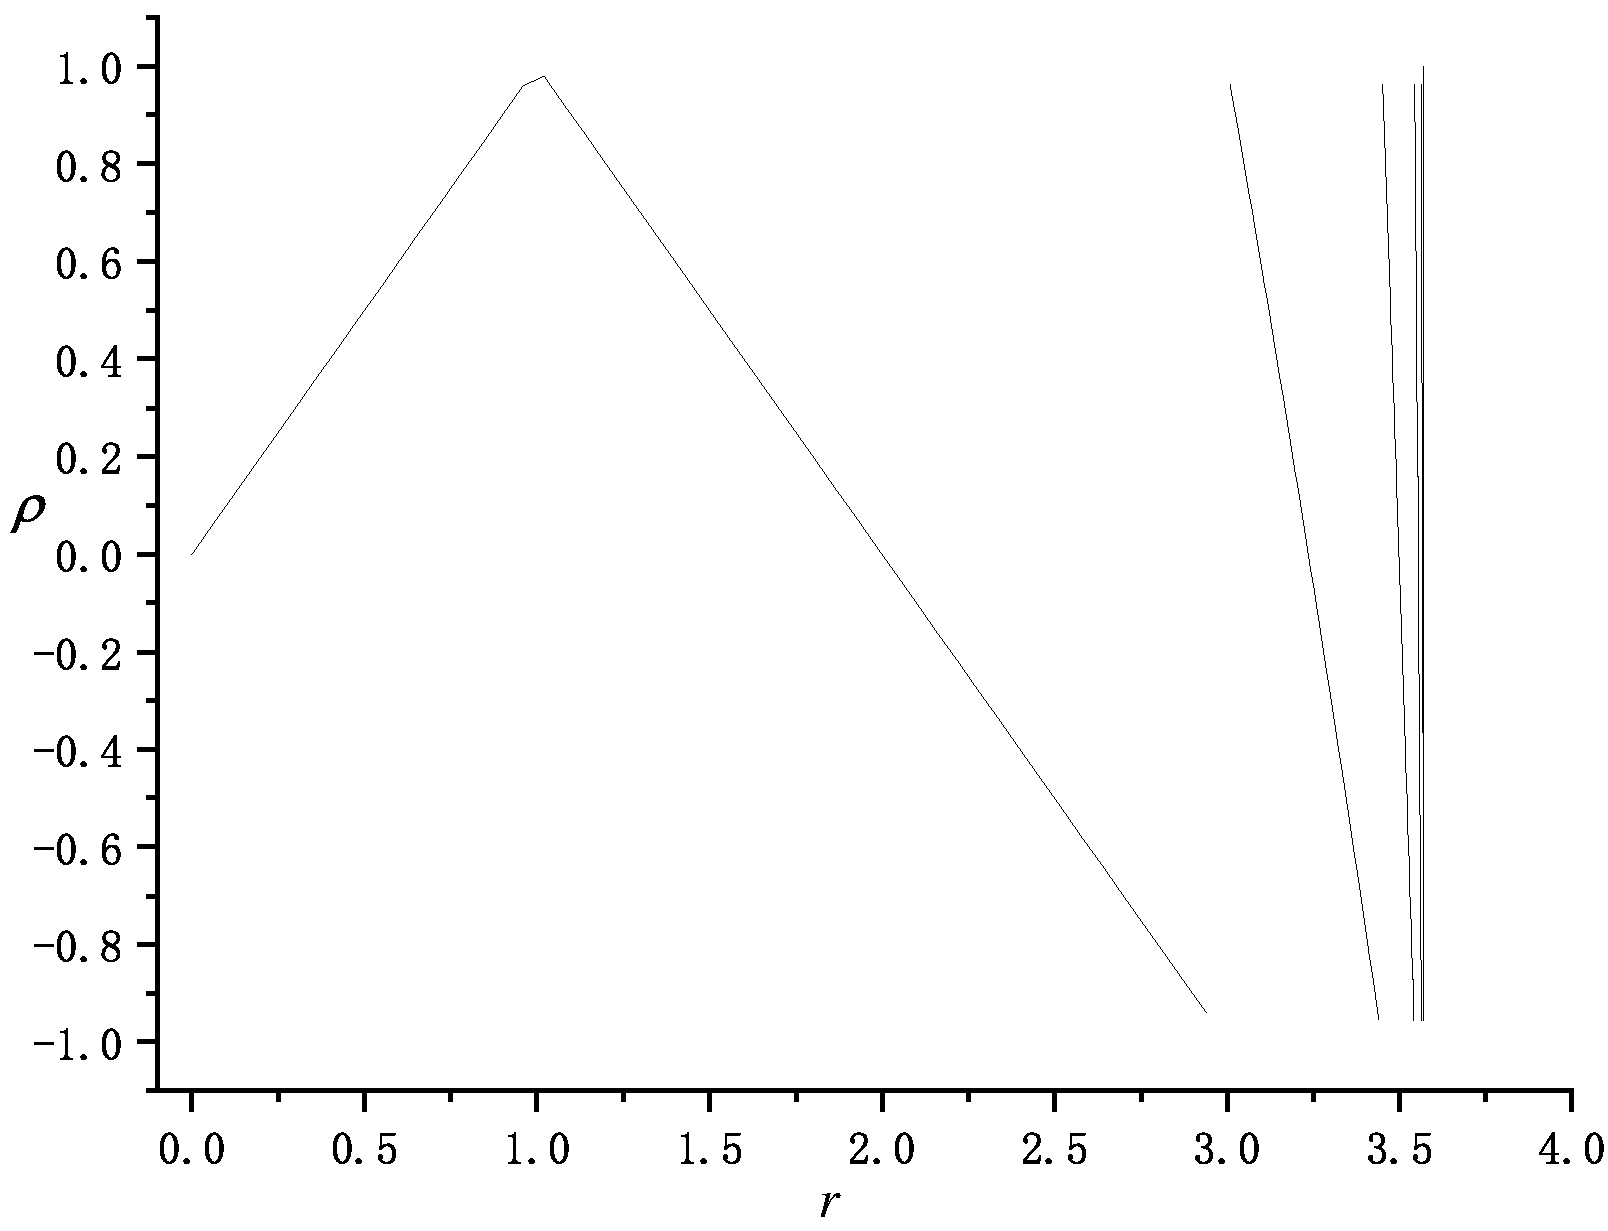
\includegraphics[width=12cm]{rho.pdf}
        \end{center}
        可以发现在一个周期区间, $\rho$是从1开始下降到-1, 而随着周期区间的逐渐减小, 下降速度越来越快;
        这也意味着在区间中间的区域收敛是最快的$(|\rho|\rightarrow 0)$, 在区间两端收敛最慢.
    \section{Question6}
        \indent 以下从左至右从上至下依次为2-8, 4-16, 8-16和16周期的图像:
        \begin{center}
            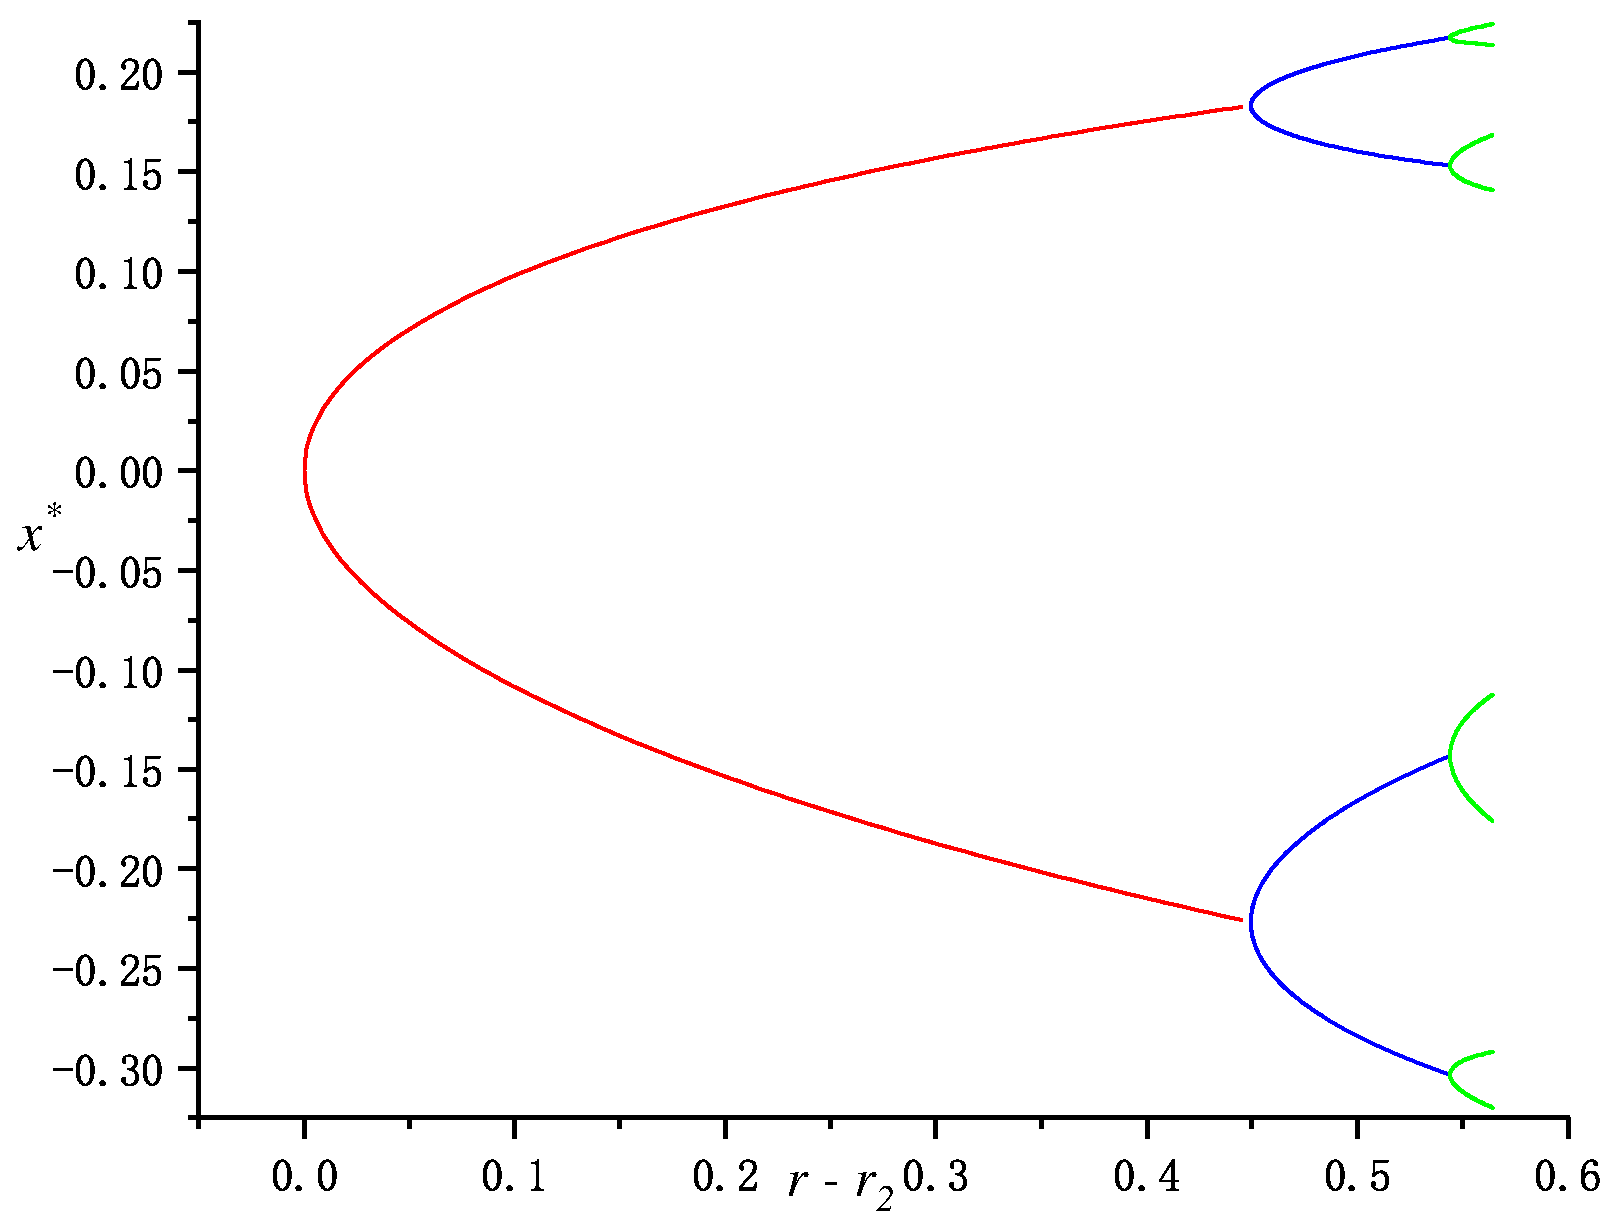
\includegraphics[width=9cm]{t2-8.pdf}
            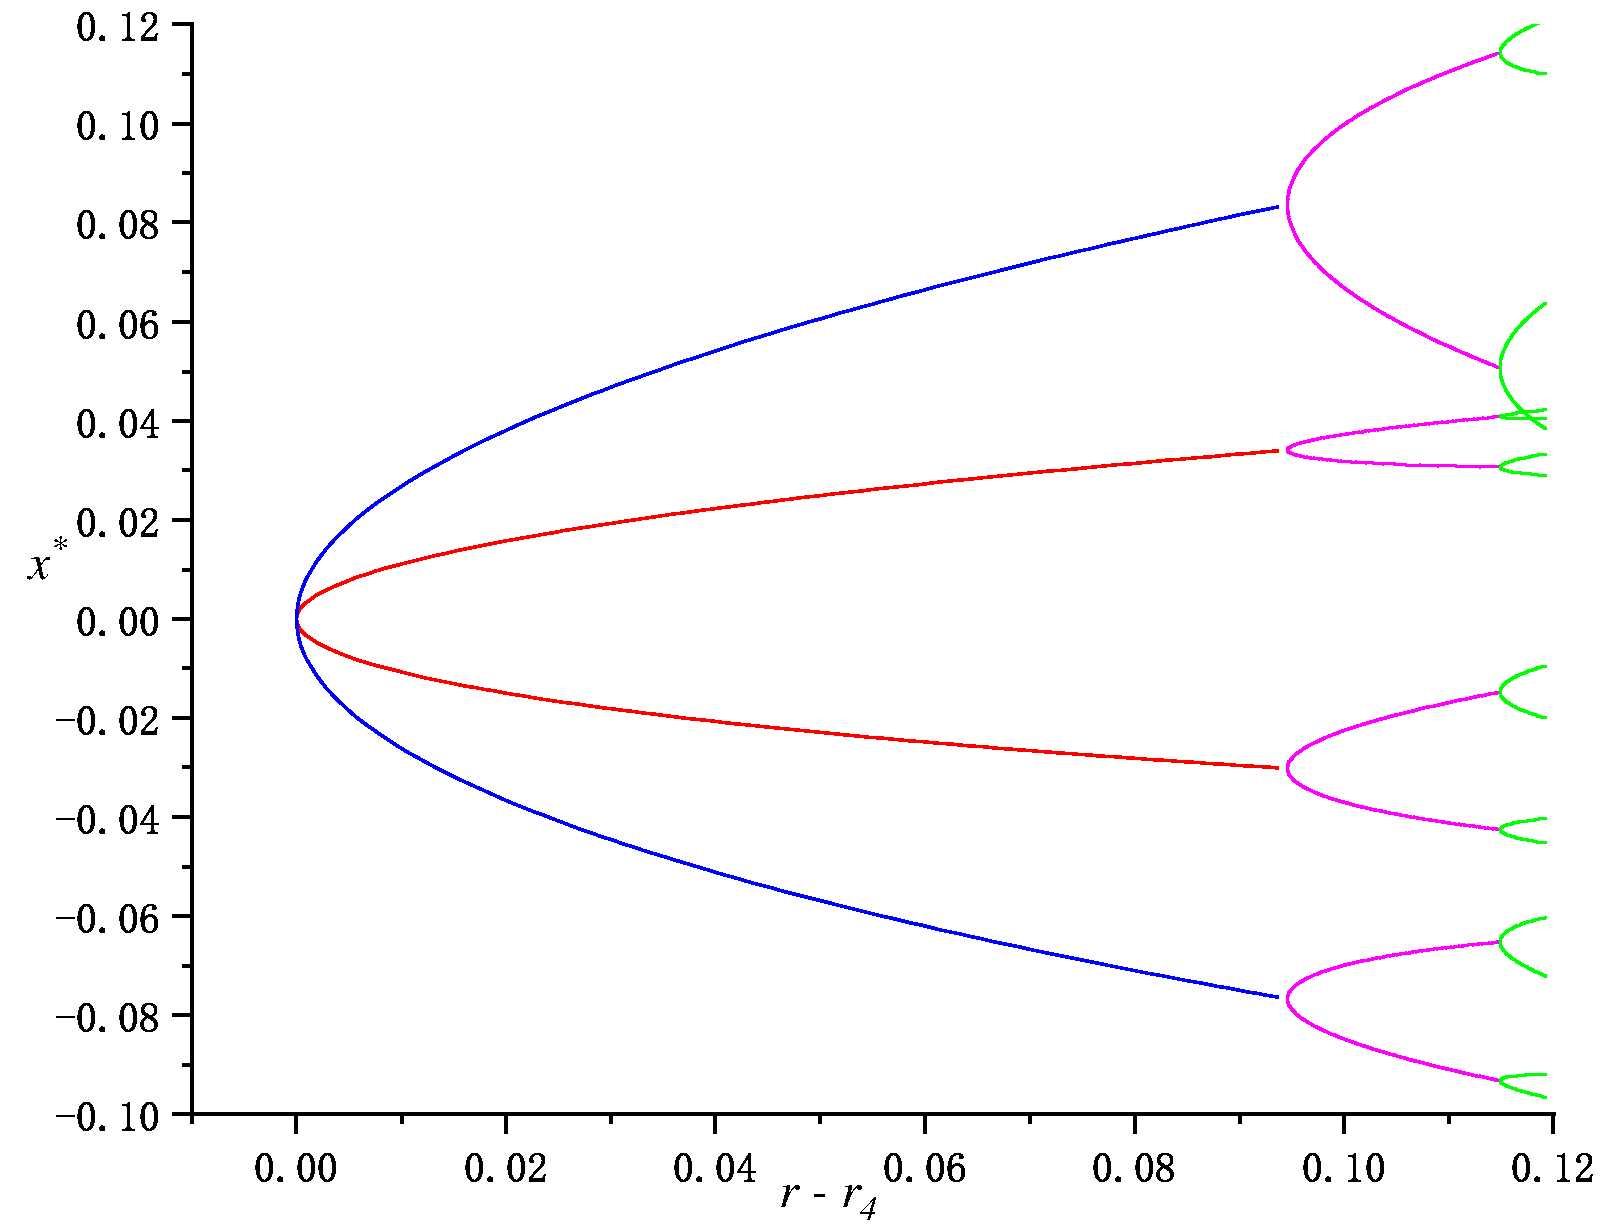
\includegraphics[width=9cm]{t4-16.pdf}
            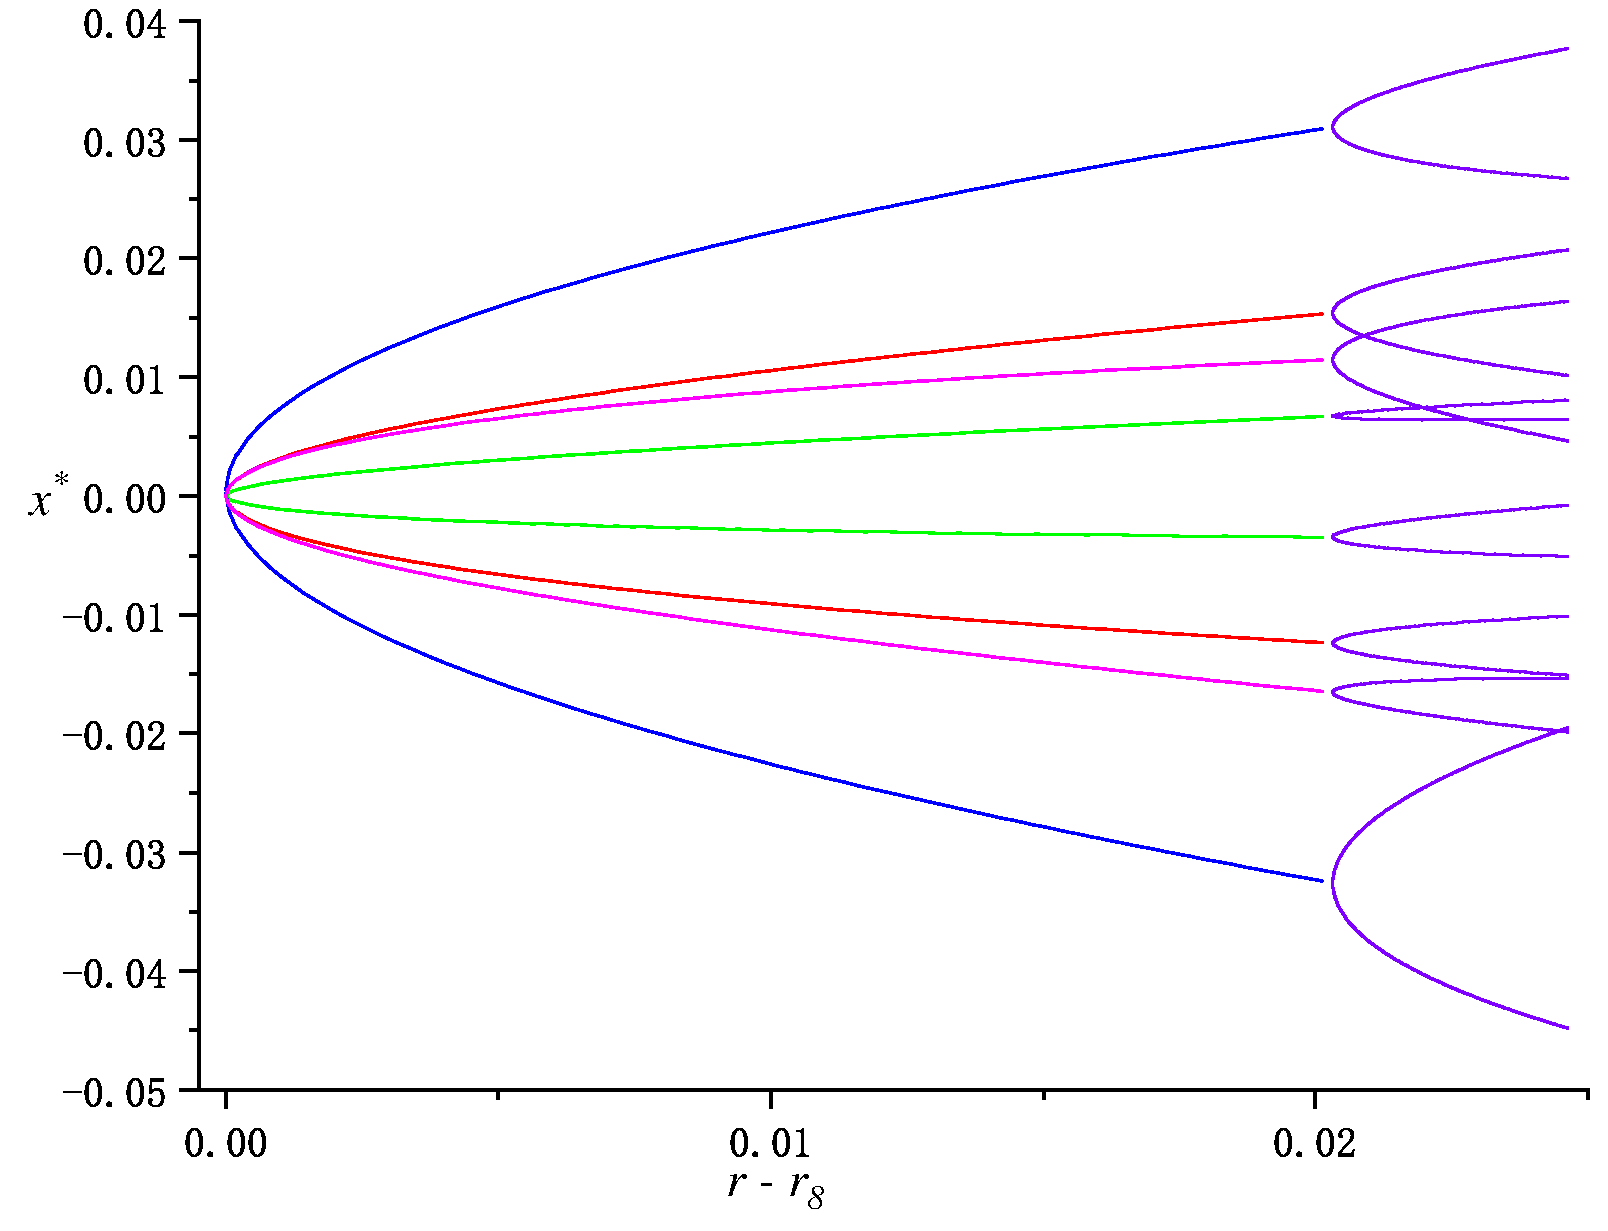
\includegraphics[width=9cm]{t8-16.pdf}
            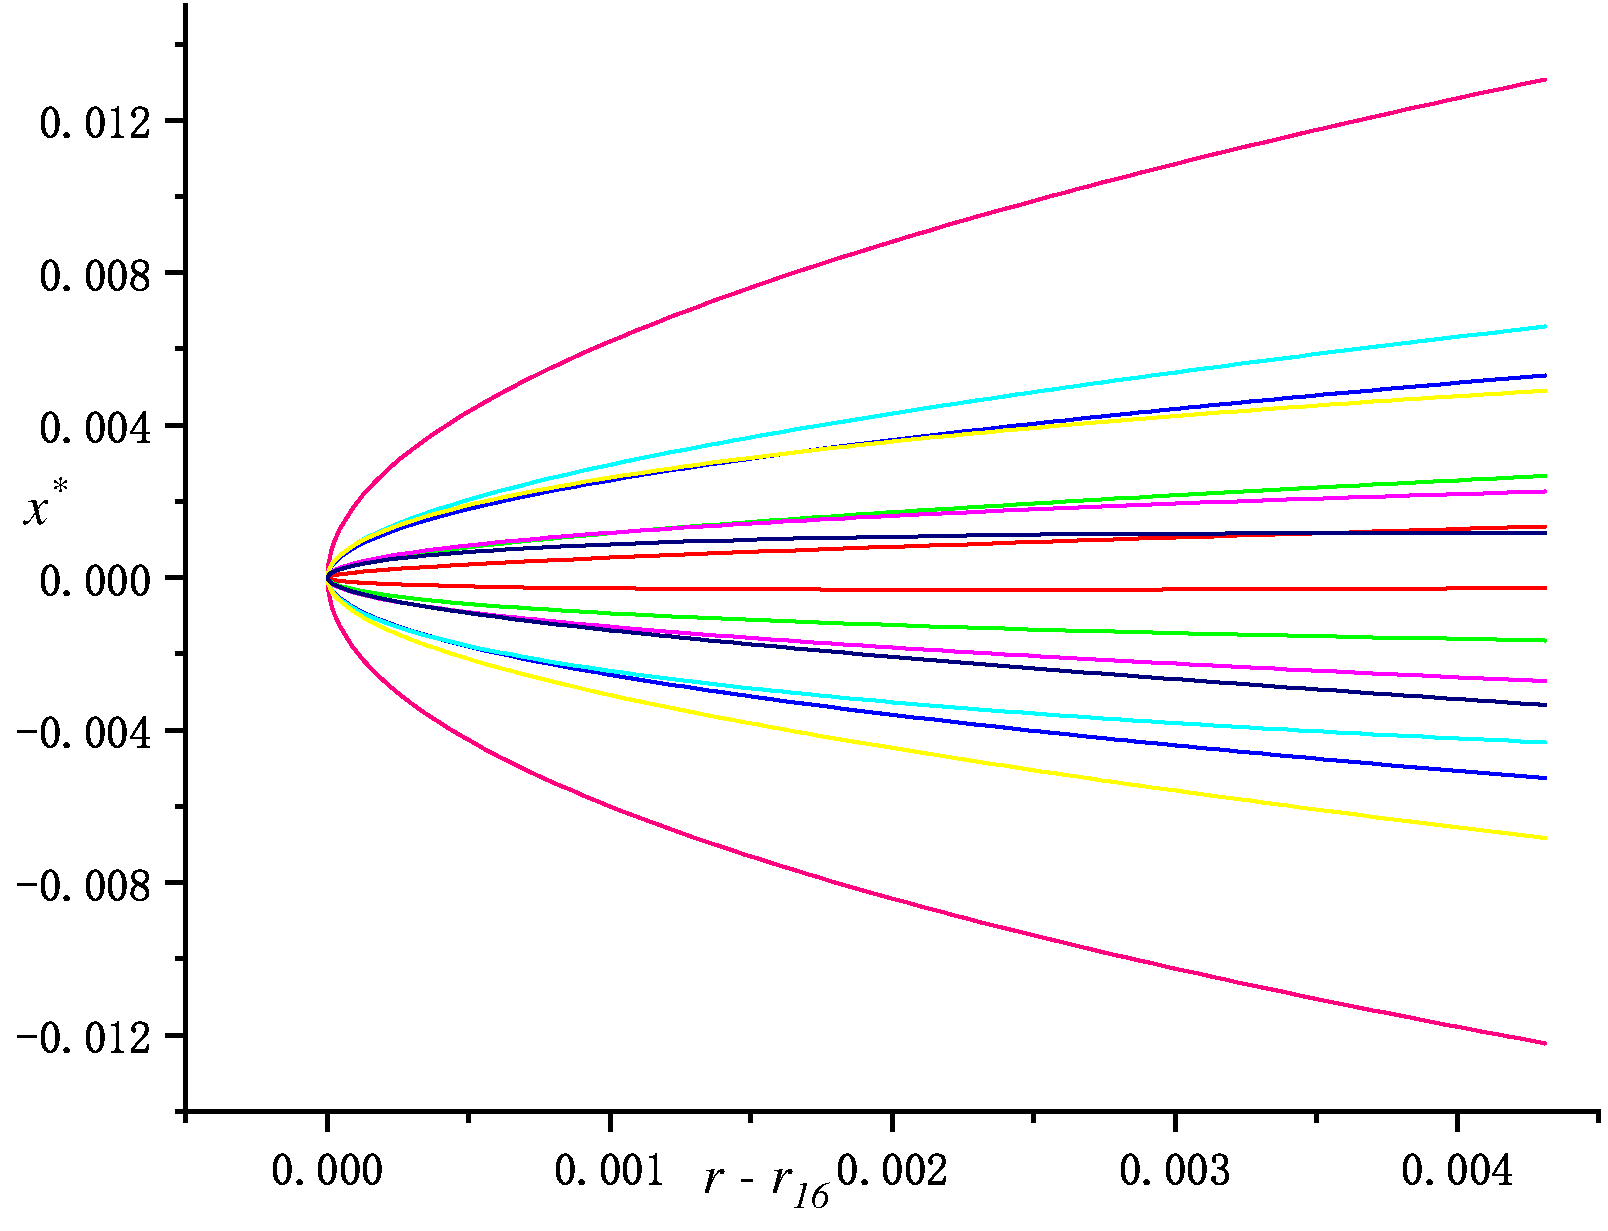
\includegraphics[width=9cm]{t16.pdf}
        \end{center}
        可以看见类似分形的结构, 但是各个分支之间并不相似.
    \section{Question7}
        \indent 将相邻$\Delta r$之比作图得到:
        \begin{center}
            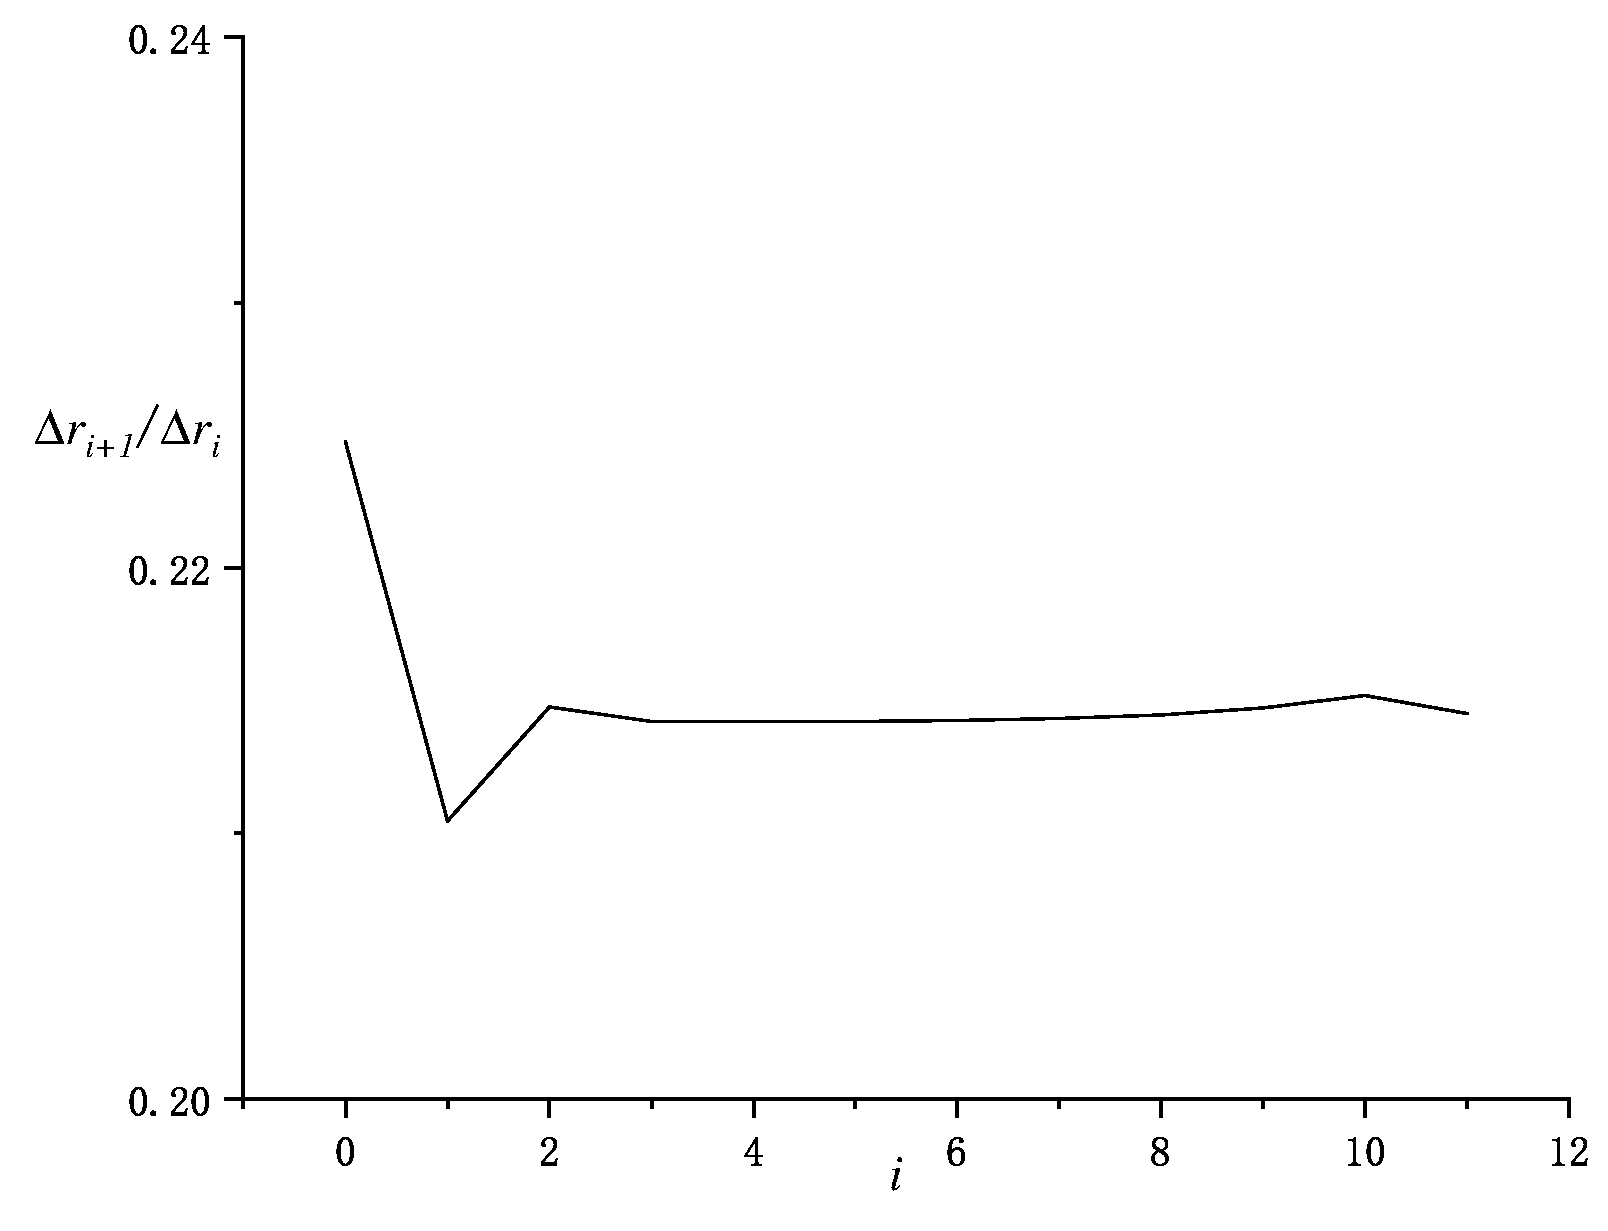
\includegraphics[width=10cm]{delta_r.pdf}
        \end{center}
        可以发现趋于一个常数$F=0.2142$, 由$F$计算等比数列求和得到$r_\infty=3.569946$.
    \section{Question8}
        \begin{equation}
            x_{n+1}=f(x_n)=4\sin^2y\cos^2y=\sin^22y
        \end{equation}
        故存在解$x_n=\sin^22^n\theta$, 其中$x_0=\sin^2\theta$. 而由于$\sin^22^n\theta(\theta\neq m\pi, m=1,2,3,...)$
        这个序列在$(0,1)$上是稠密的, 即不存在稳定的振荡周期.
    \section{Question9}
        \indent 选取$f(x)=\sin x$得到以下结果:\\
        \indent 选取$r=0.5$和$r=1.5$时不同初值的迭代结果:
        \begin{center}
            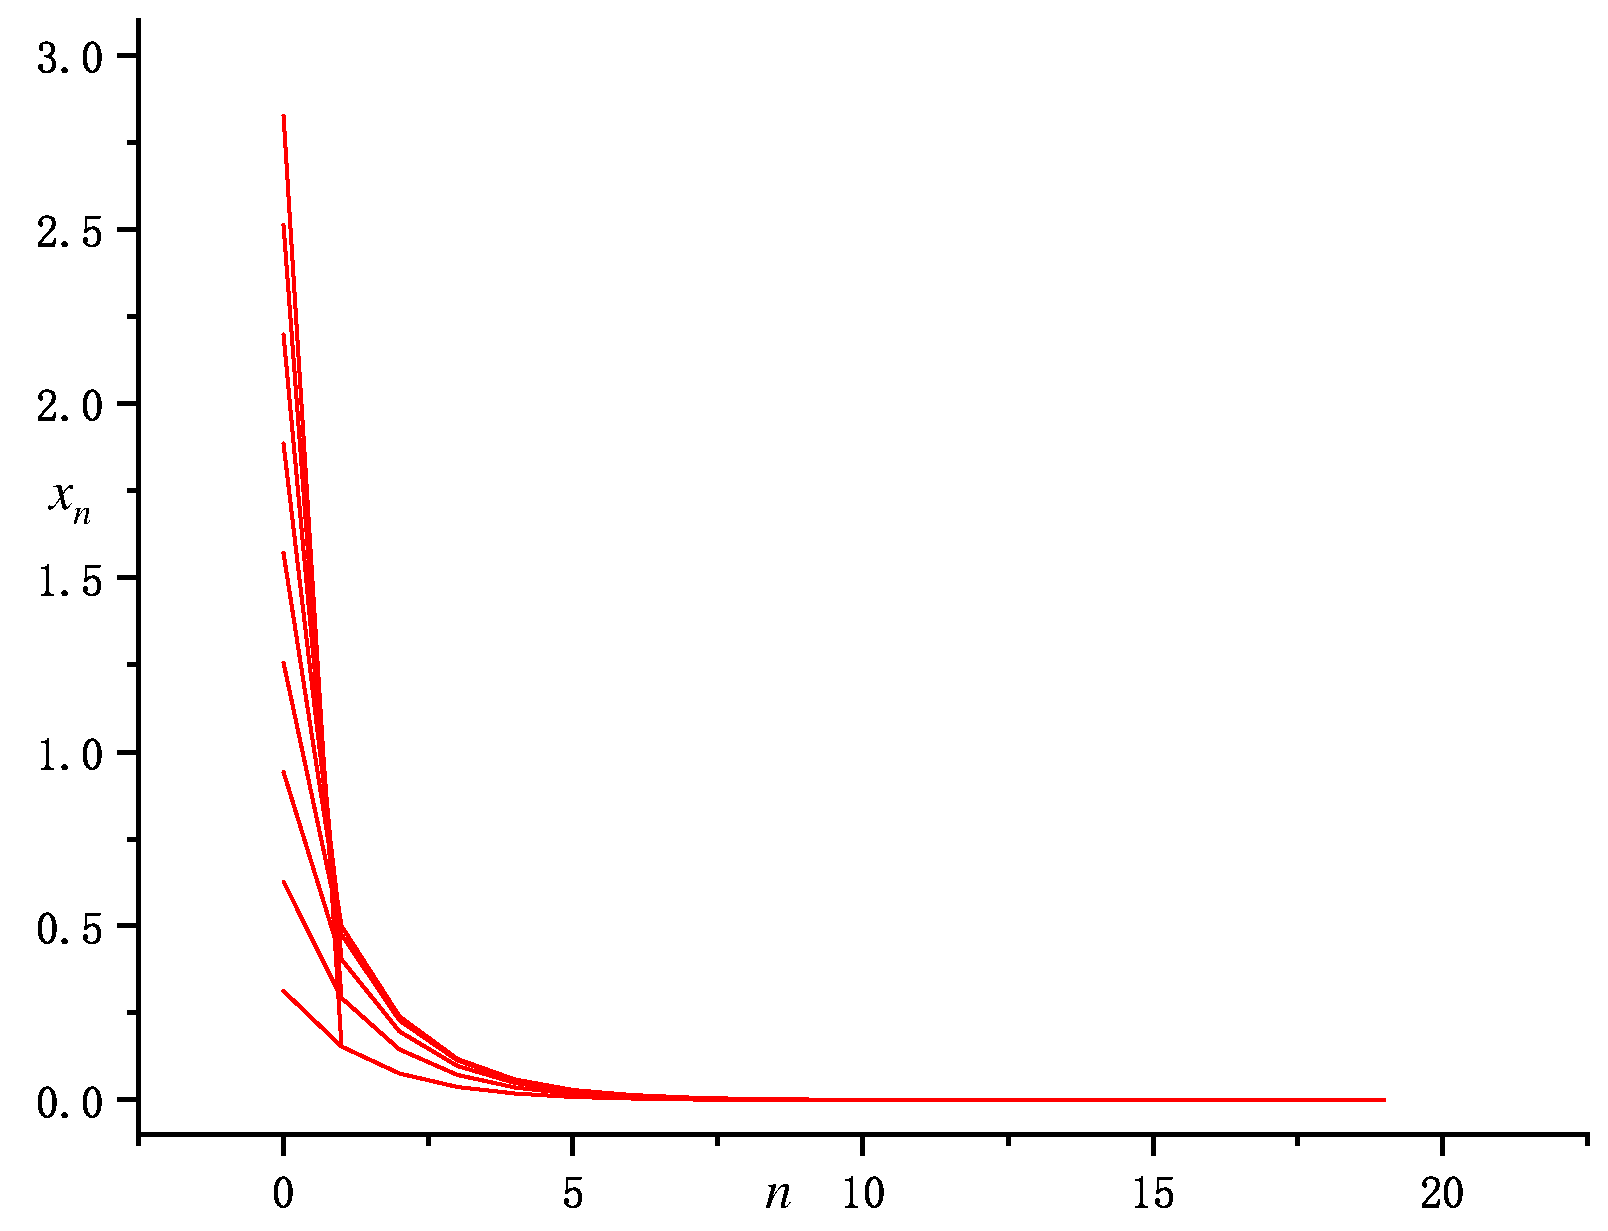
\includegraphics[width=9cm]{q9/r0_5.pdf}
            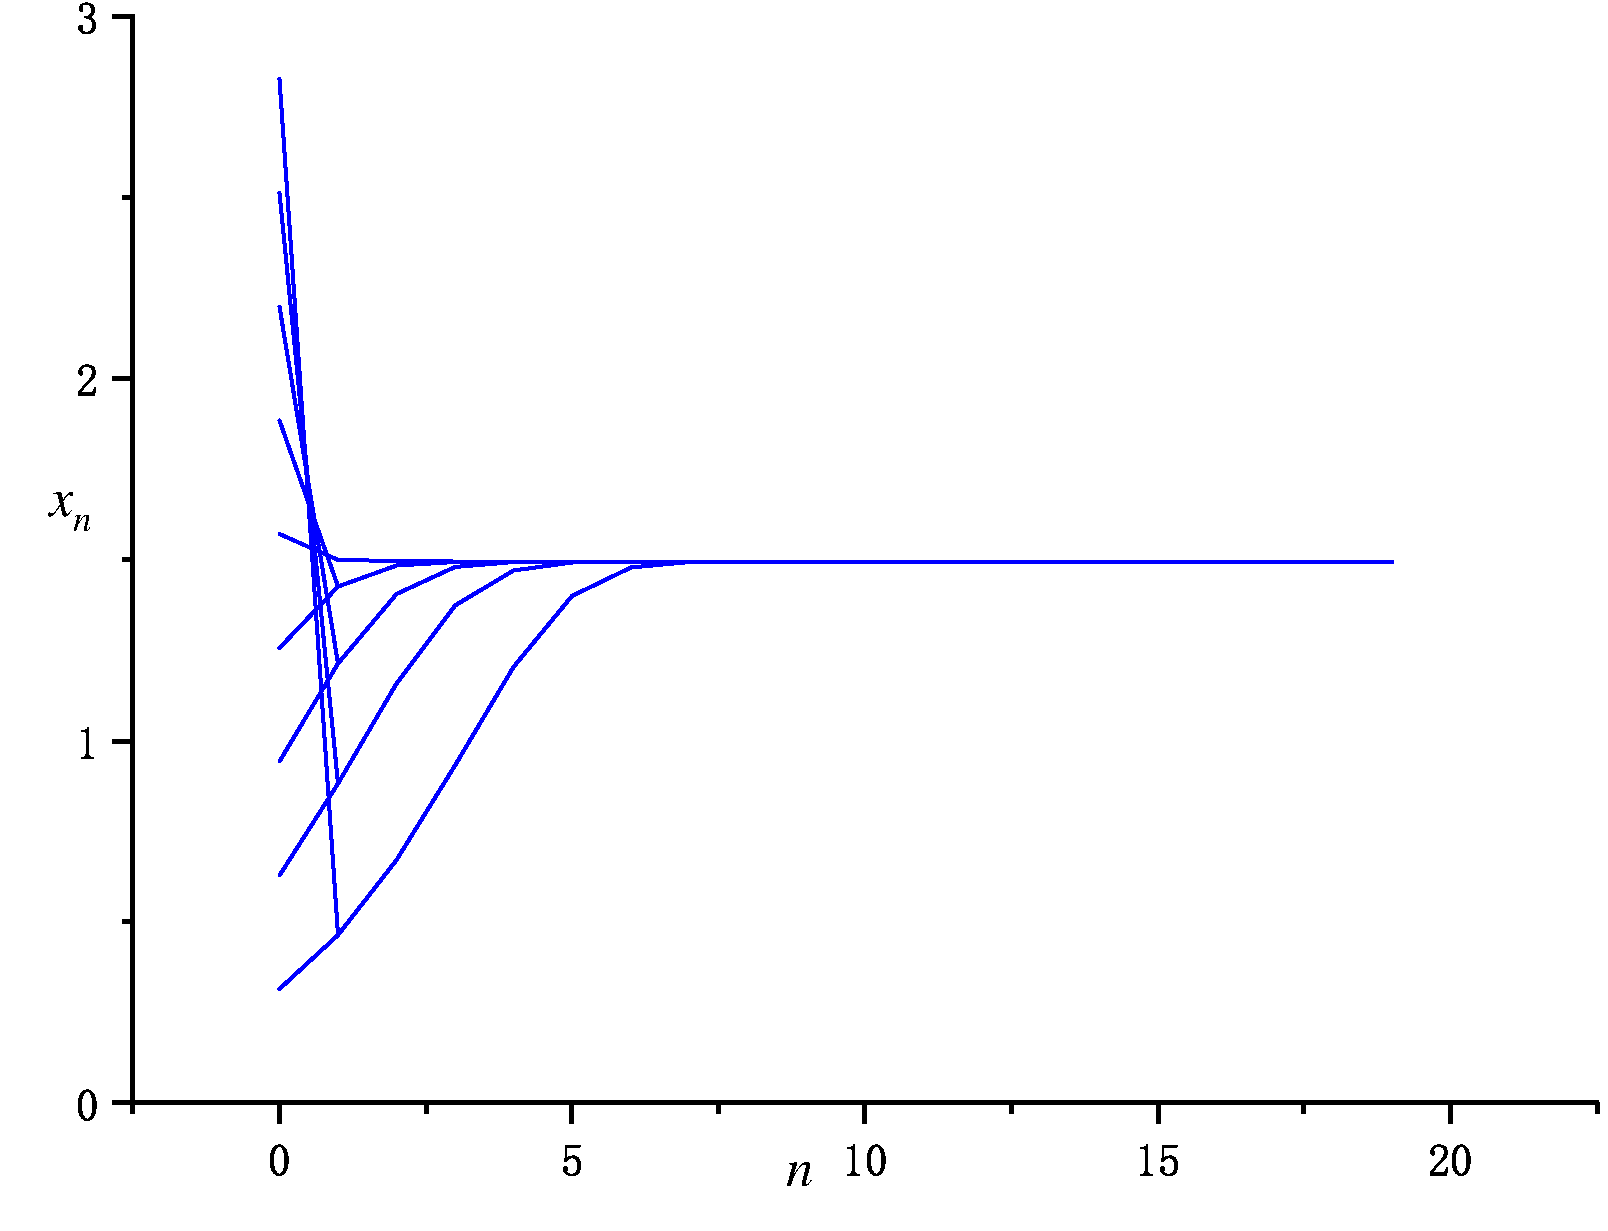
\includegraphics[width=9cm]{q9/r1_5.pdf}
        \end{center}
        \indent 选取$r=2.3616$(第一个分支点的$r+0.1$)时:
        \begin{center}
            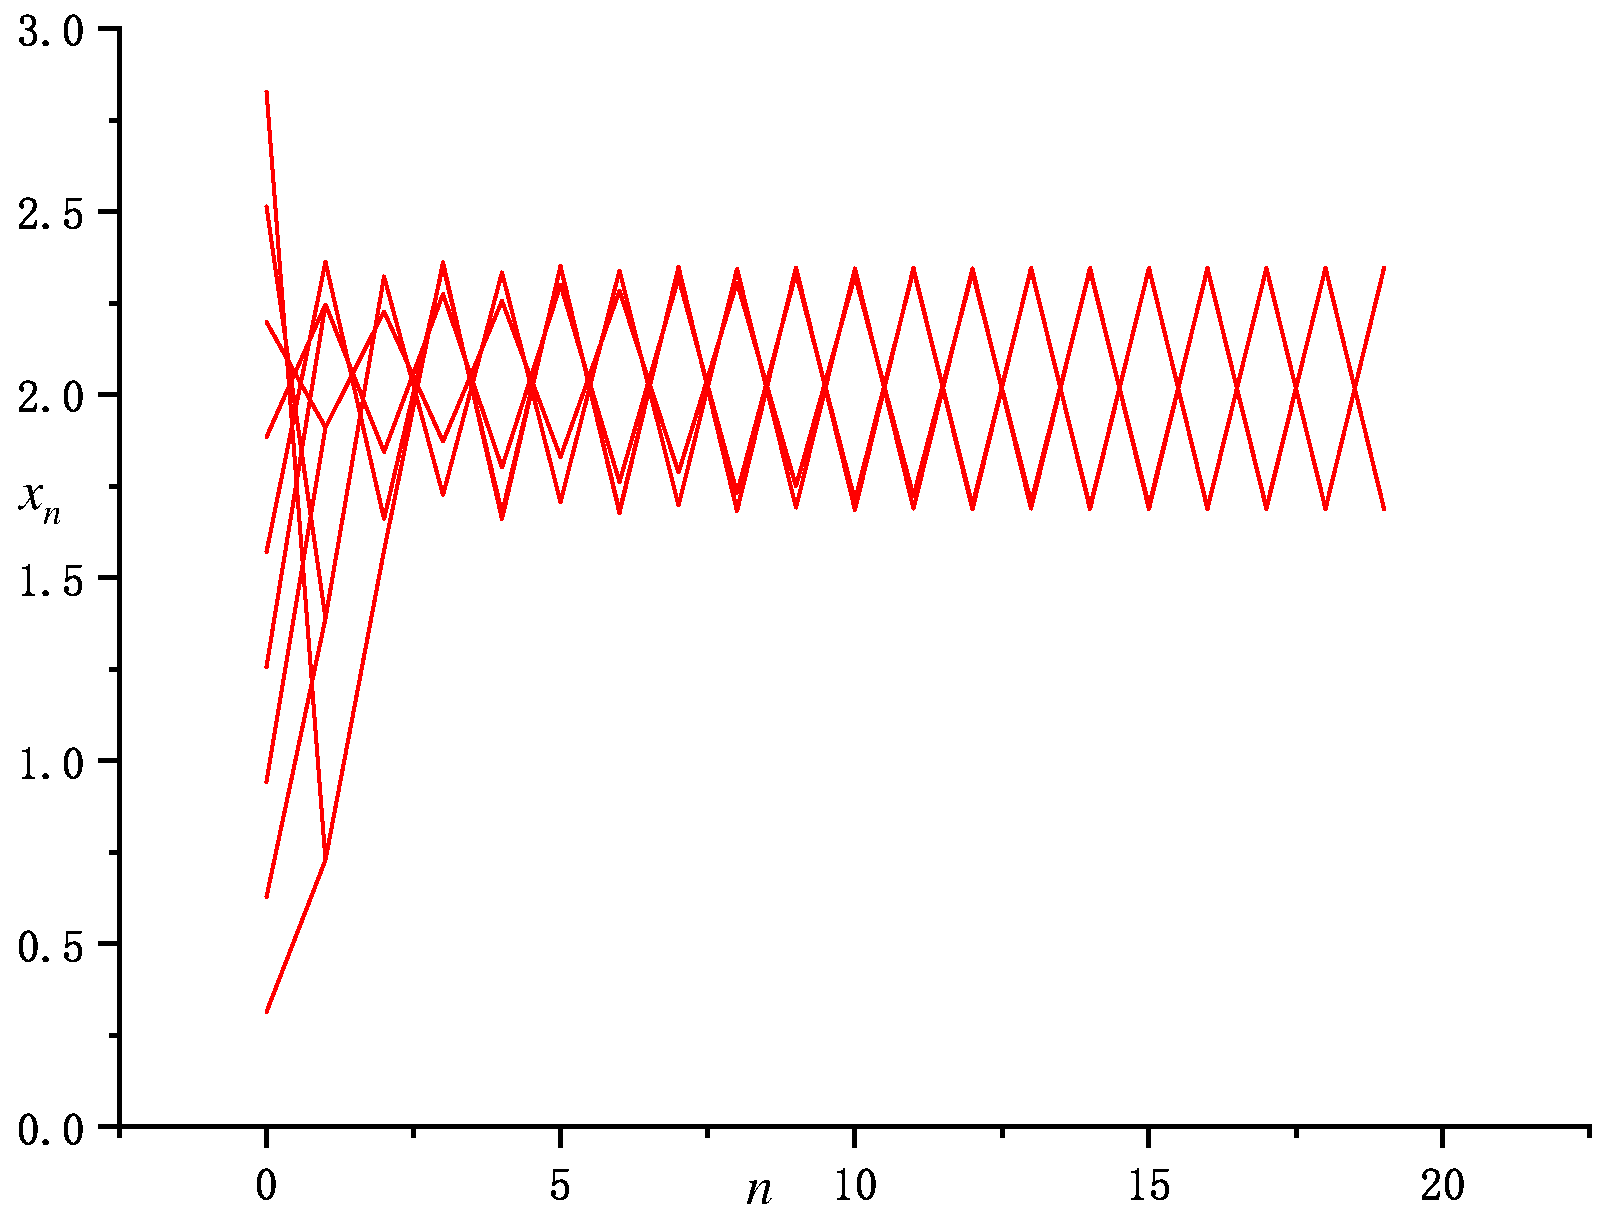
\includegraphics[width=13cm]{q9/r2_36.pdf}
        \end{center}
        \indent $x^*-r$的关系图:
        \begin{center}
            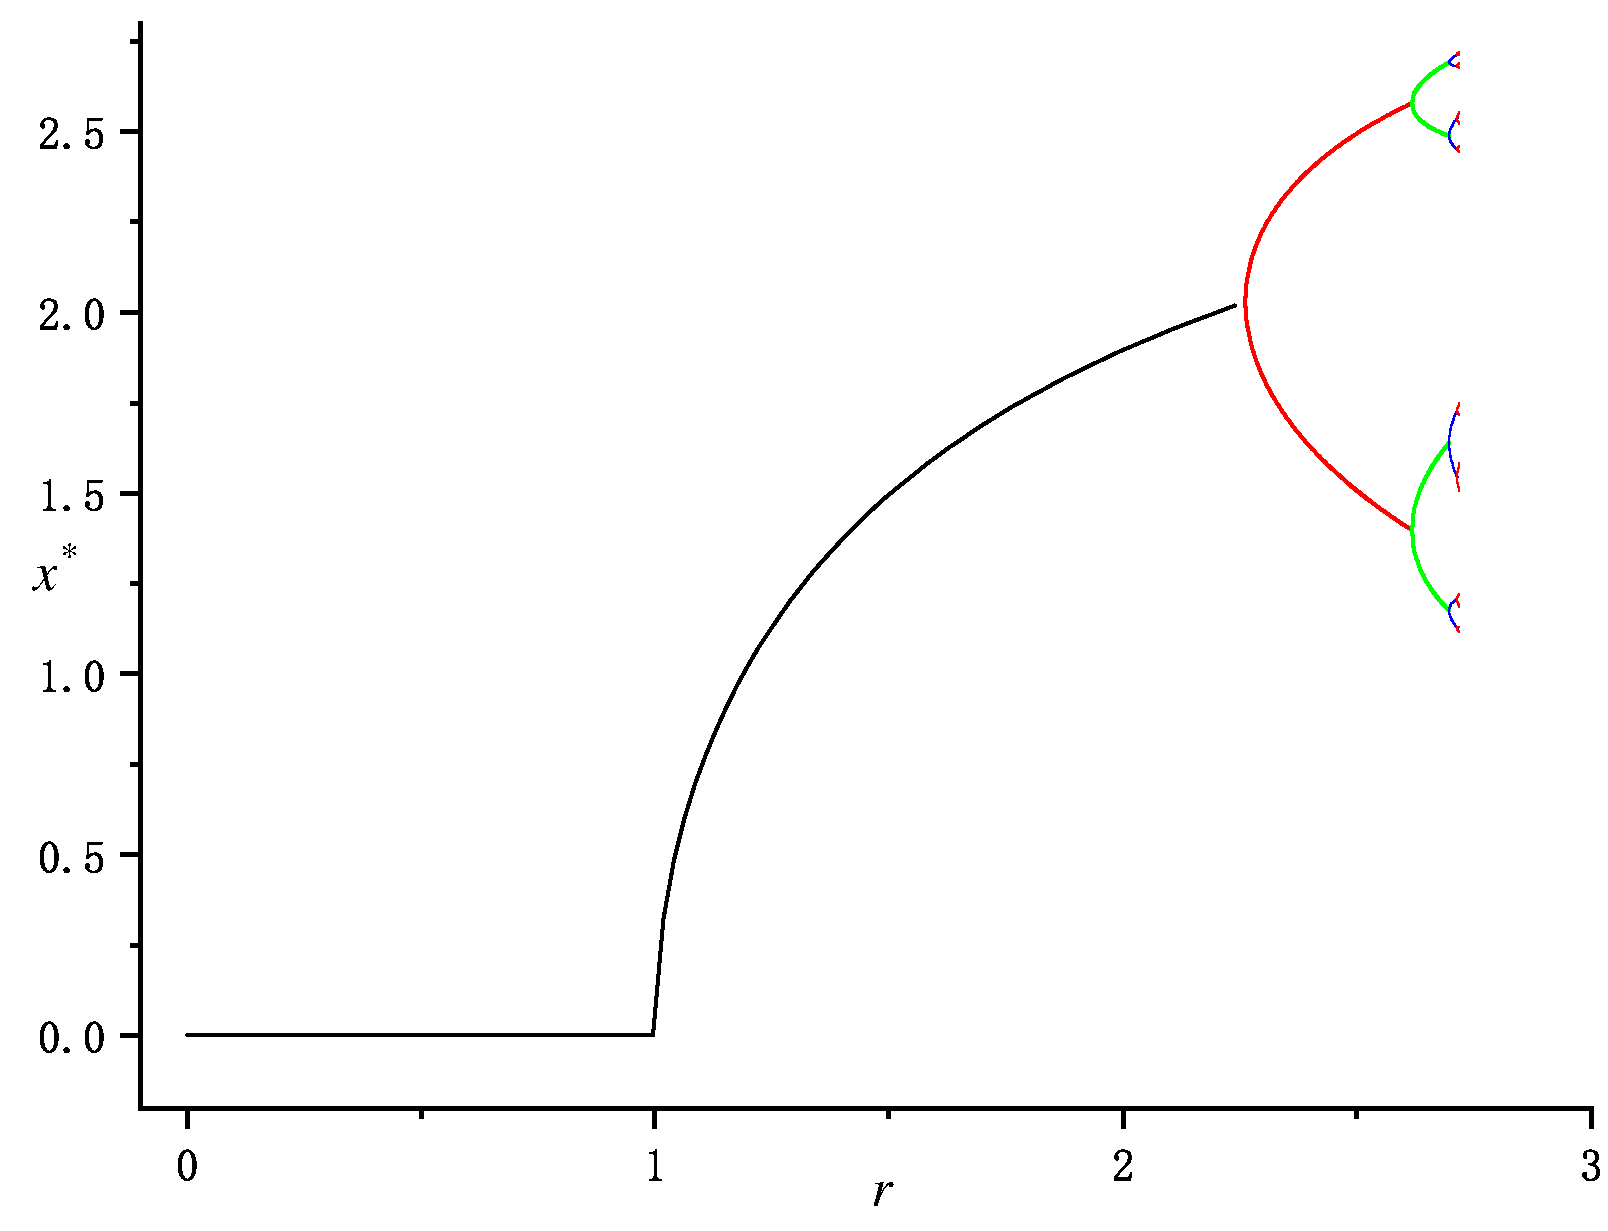
\includegraphics[width=13cm]{q9/t1-16.pdf}
        \end{center}
        \indent 平均收敛速度:
        \begin{center}
            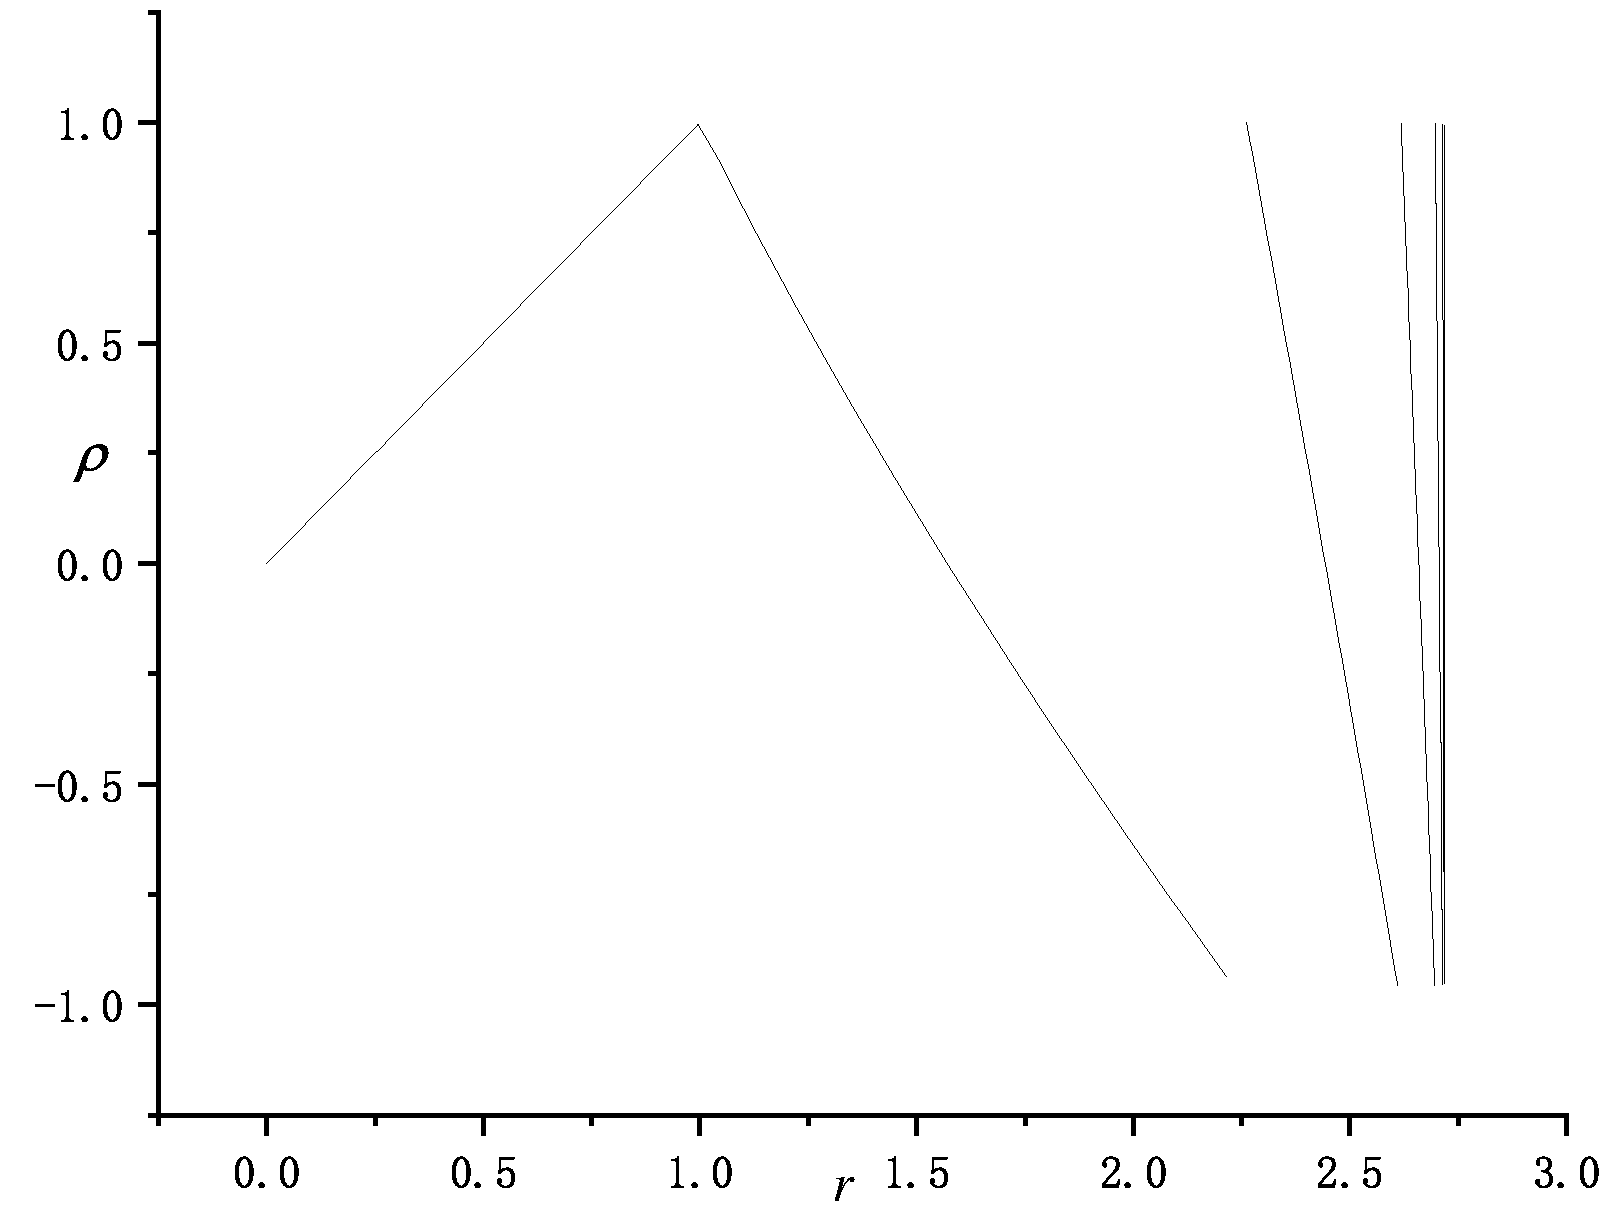
\includegraphics[width=13cm]{q9/rho.pdf}
        \end{center}
        \indent 相邻$\Delta r$之比:
        \begin{center}
            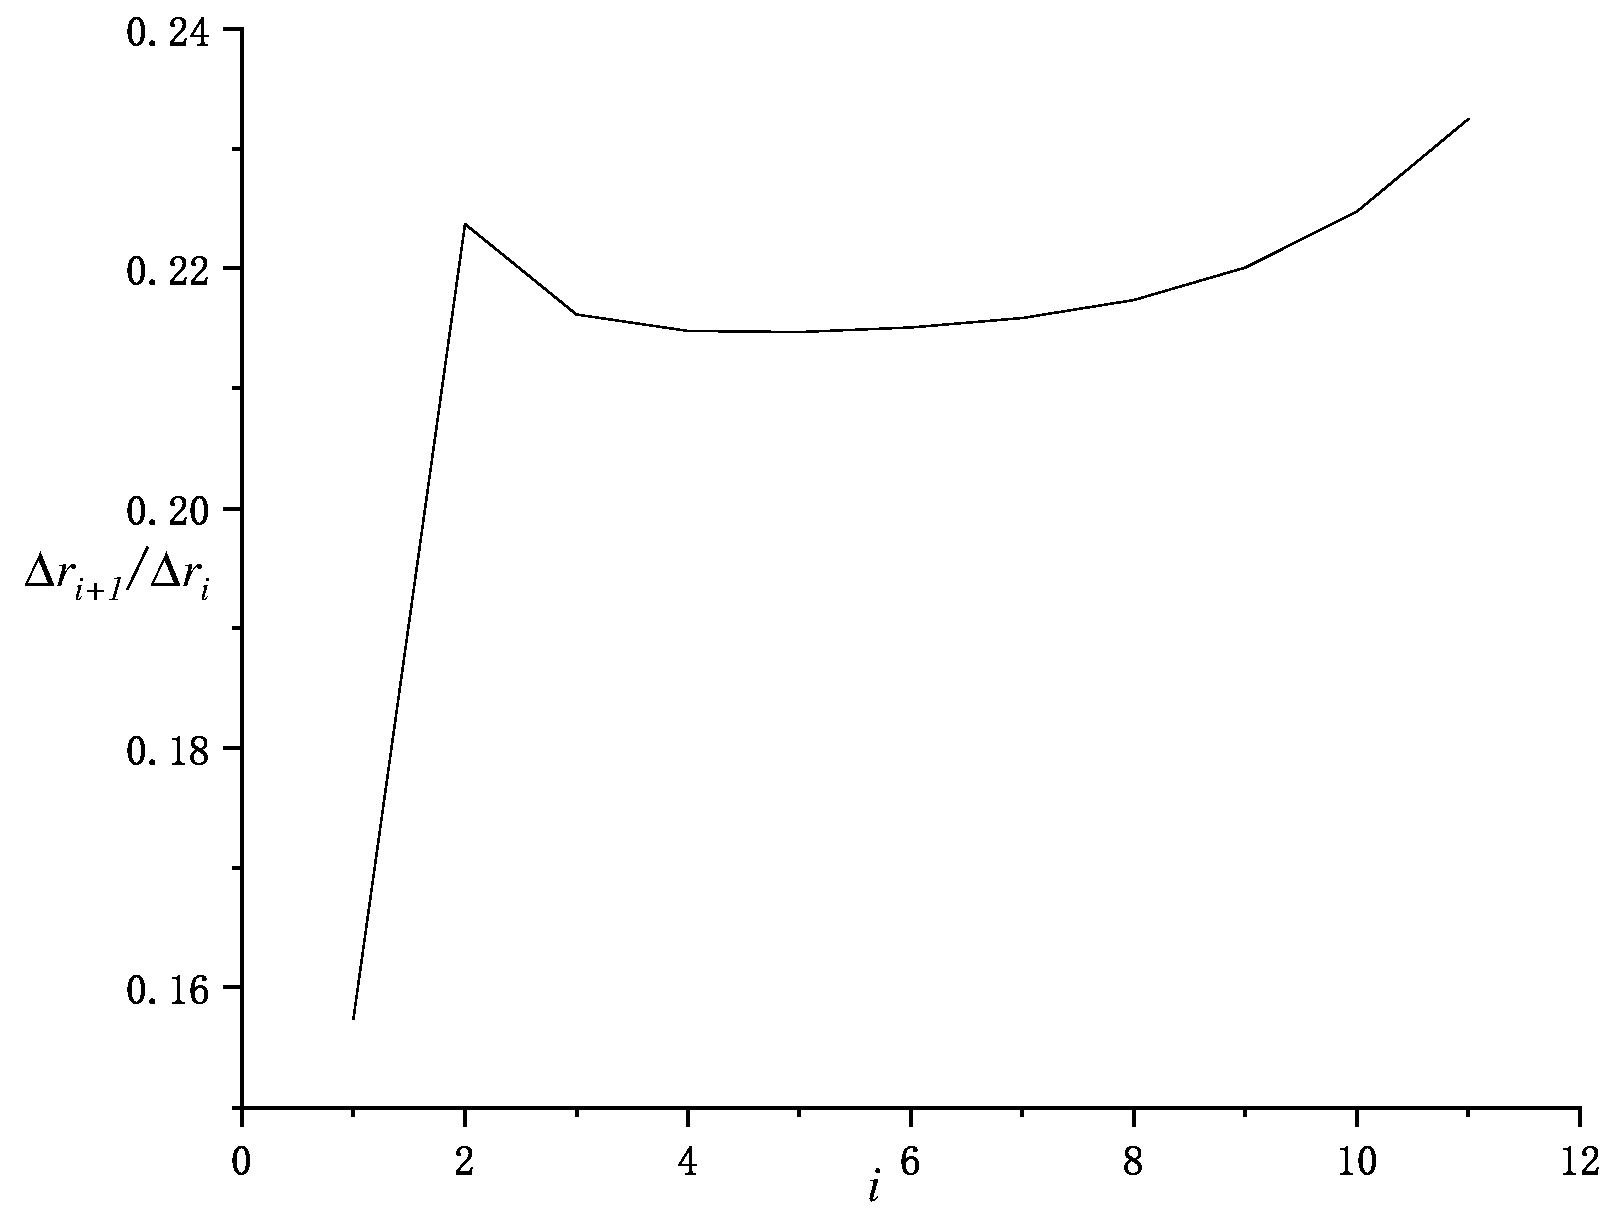
\includegraphics[width=13cm]{q9/delta_r.pdf}
        \end{center}
        可以发现这个比值并不是像之前一样趋于一个常数值, 中间的最小值为0.21473, 近似等于之前的$F$.
        可以这样解释: 实际计算中我发现在分叉点附近后半周期与前半周期的差值非常小,
        在$10^{-10}$以下, 而在$10^{-10}$之后这个差值会迅速增大,
        所以我就按照$10^{-10}$为分界线把前后2个周期区间分开,
        现在看来这种分开方式在周期数很大的时候可能是不准确的.
\end{document}